%\documentclass[preprint]{aa}
\documentclass[onecolumn, 12pt]{aa}
\pdfoutput=1

\bibliographystyle{aa}
%\AuthorCallLimit=200


\usepackage{amsmath}
\usepackage{amsfonts}
\usepackage{dsfont}
\usepackage{amsxtra}
\usepackage{hyperref}
\usepackage{amssymb}
\usepackage{upgreek}

\usepackage{multirow}
\usepackage{url}

\usepackage{graphicx,epsfig}
%\usepackage{dcolumn}
%\usepackage{bm}
%\usepackage{ulem}

\usepackage{xspace} 

\usepackage{color}
\usepackage{xcolor}

\usepackage[mathlines, switch]{lineno}
\linenumbers
\usepackage{comment}

\usepackage{subcaption}
\usepackage{graphicx} % for subfigures
\usepackage{siunitx} % for units

\renewcommand{\baselinestretch}{1.4}
\setlength\tabcolsep{3 pt}

\setlength{\textwidth}{16cm} 
%\setlength{\textheight}{24.cm}
%\setlength{\topmargin}{-1.5cm}
\setlength{\oddsidemargin}{-0.0cm}
\setlength{\evensidemargin}{-0.0cm}

\newcommand{\be}{\begin{equation}}
\newcommand{\ee}{\end{equation}}
\newcommand{\bea}{\begin{eqnarray}}
\newcommand{\eea}{\end{eqnarray}}
\newcommand{\beaa}{\begin{eqnarray*}}
\newcommand{\eeaa}{\end{eqnarray*}}
\newcommand{\ba}{\begin{array}}
\newcommand{\ea}{\end{array}}
\newcommand{\bi}{\begin{itemize}}
\newcommand{\ei}{\end{itemize}}
\newcommand{\ben}{\begin{enumerate}}
\newcommand{\een}{\end{enumerate}}

\newcommand{\bra}{\langle}
\newcommand{\ket}{\rangle}
\newcommand{\ra}{\rightarrow}
\newcommand{\lra}{\longrightarrow}
\newcommand{\overar}{\overrightarrow}
\newcommand{\wt}{\widetilde}
\newcommand{\td}{\tilde}


\newcommand{\lb}{\label}
\newcommand{\g}{\ensuremath{\gamma}\xspace}
\newcommand{\G}{\Gamma}
\newcommand{\e}{\epsilon}
\newcommand{\al}{\alpha}
\newcommand{\bt}{\beta}
\newcommand{\p}{\partial}
\newcommand{\dl}{\delta}
\newcommand{\Dl}{\Delta}
\newcommand{\ld}{\lambda}
\newcommand{\Ld}{\Lambda}
\newcommand{\vp}{\varphi}
\newcommand{\te}{\theta}
\newcommand{\Om}{\Omega}
\newcommand{\om}{\omega}
\newcommand{\sm}{\sigma}
\newcommand{\Sm}{\Sigma}

\newcommand{\A}{{\rm A}}
\newcommand{\B}{{\rm B}}
\newcommand{\U}{{\rm U}}
\newcommand{\F}{{\rm F}}
\newcommand{\SU}{{\rm SU}}
\newcommand{\Tr}{{\rm Tr}}
\newcommand{\Hom}{{\rm Hom}}

\newcommand{\FF}{{\mathsf F}}

\newcommand{\mcE}{{\mathcal{E}}}
\newcommand{\N}{{\mathcal{N}}}
\newcommand{\D}{{\mathcal{D}}}
\newcommand{\La}{{\mathcal{L}}}
\newcommand{\OO}{{\mathcal{O}}}
\newcommand{\M}{{\mathcal{M}}}


\newcommand{\mbE}{{\mathbb{E}}}
\newcommand{\Z}{{\mathbb{Z}}}
\newcommand{\R}{{\mathbb{R}}}
\newcommand{\C}{{\mathbb{C}}}
\newcommand{\NN}{{\mathbb{N}}}
\newcommand{\PP}{{\mathbb{C}}{\rm P}}

\newcommand{\HH}{{\mathcal{H}}}
\newcommand{\Hd}{{\mathcal{H}}^*}

\newcommand{\HI}{H~\textsc{i}\xspace}
\newcommand{\Htwo}{$\mathrm{H}_2$\xspace}
\newcommand{\hi}{$\mathrm{H\,\scriptstyle{I}}$\xspace}
\newcommand{\hii}{$\mathrm{H\,\scriptstyle{II}}$\xspace}
\newcommand{\hd}{$\mathrm{H}_2$\xspace}
\newcommand{\xco}{$X_\mathrm{CO}$\xspace}

\newcommand{\vx}{{\bf x}}

\newcommand{\Fermi}{\textsl{Fermi}\xspace}
\newcommand{\LAT}{\textsl{LAT}\xspace}
\newcommand{\WMAP}{\textsl{WMAP}\xspace}
\newcommand{\Planck}{\textsl{Planck}\xspace}
\newcommand{\Suzaku}{\textsl{Suzaku}\xspace}
\newcommand{\DAMPE}{\textsl{DAMPE}\xspace}
\newcommand{\Healpix}{HEALPix\xspace}


\newcommand{\SM}{Sample Model\xspace}

\newcommand{\sigmav}{\ensuremath{\langle \sigma v \rangle}\xspace}
\newcommand{\bbbar}{\ensuremath{b \bar b}\xspace}
\newcommand{\tautau}{\ensuremath{\tau^{+}\tau^{-}}\xspace}
\newcommand{\relic}{\ensuremath{2.2\times10^{-26}\cm^{3}\second^{-1}}\xspace}
\newcommand{\beff}{\ensuremath{b_{\rm eff}}\xspace}
\newcommand{\DM}{\ensuremath{\mathrm{DM}}}
\newcommand{\mDM}{\ensuremath{m_\DM}\xspace}


% local options
\newcommand{\onepic}{0.49}
\newcommand{\twopic}{0.49}
\newcommand{\twopicsp}{0.45}
\newcommand{\threepic}{0.33}
%\newcommand{\threepic}{0.18}
\newcommand{\fourpic}{0.28}
\newcommand{\twopicwca}{0.35}

\newcommand{\cmap}{_afmhot}


\newcommand{\red}{\textcolor{red}}
\newcommand{\blue}{\textcolor{blue}}
\definecolor{darkgreen}{rgb}{0.0, 0.7, 0.0}
\newcommand{\green}{\textcolor{darkgreen}}

\newcommand{\dima}[1]{\textcolor{blue}{(Dima: #1)}}
\newcommand{\Laura}[1]{\textcolor{red}{(Laura: #1)}}
\newcommand{\cmt}[1]{}


\newcommand{\low}{\text{low}}
\newcommand{\model}{\text{model}}
\newcommand{\east}{\text{east}}
\newcommand{\west}{\text{west}}
\newcommand{\de}{\text{d}}
\newcommand{\IC}{\text{IC}}
\newcommand{\ISRF}{\text{ISRF}}
\newcommand{\el}{\text{e}}
\newcommand{\pr}{\text{p}}
\newcommand{\cut}{\text{cut}}
\newcommand{\eto}{\text{e}}
\newcommand{\Hy}{\text{H}}
\newcommand{\tot}{\text{tot}}

% local options

\begin{document} 


   \title{Hard and bright gamma-ray emission at the base of the \Fermi bubbles}


   %\subtitle{}

   \author{L. Herold \thanks{\email{laura.herold@fau.de}}
          \inst{1}
          \and
          D. Malyshev \thanks{\email{dmitry.malyshev@fau.de}}
          \inst{1}
          }

   \institute{
             Erlangen Centre for Astroparticle Physics, Erwin-Rommel-Str. 1, Erlangen, Germany
             }

   \date{Received August 15, 2018; accepted November 16, 2018}

% \abstract{}{}{}{}{} 
% 5 {} token are mandatory
 
\abstract
% context heading (optional)
% {} leave it empty if necessary
{The \Fermi bubbles (FBs) are large gamma-ray emitting lobes extending up to $55^\circ$ in latitude above and below the Galactic center (GC).
Although the FBs were discovered 8 years ago, their origin and the nature of the gamma-ray emission are still unresolved.
Understanding the properties of the FBs near the Galactic plane may provide a clue to their origin.
Previous analyses of the gamma-ray emission at the base of the FBs, what remains after subtraction of Galactic foregrounds,
have shown an increased intensity compared to the FBs at high latitudes,
a power-law spectrum without a significant cutoff up to approximately 1 TeV,
and a displacement of the emission to negative longitudes relative to the GC.
}
% aims heading (mandatory)
{We analyze 9 years of  \Fermi Large Area Telescope data in order to study in more detail than the previous analyses
the gamma-ray emission at the base of the FBs,
especially at energies above 10 GeV.
}
% methods heading (mandatory)
{ We use a template analysis method to model the observed gamma-ray data
and calculate the residual emission after subtraction of the expected foreground and background emission components.
Since there are large uncertainties in the determination of the Galactic gamma-ray emission towards the GC,
we use several methods to derive Galactic gamma-ray diffuse emission as well as the contribution from point sources
in order to estimate the uncertainties in the emission at the base of the FBs.
}
% results heading (mandatory)
{We confirm that the gamma-ray emission at the base of the FBs is well described by a simple power law up to 1 TeV energies.
The 95\% confidence lower limit on the cutoff energy is about 500 GeV.
It has larger intensity than the FBs emission at high latitudes and is shifted to the west (negative longitudes) from the GC.
If the emission at the base of the FBs is indeed connected to the high-latitude FBs, 
then the shift of the emission to negative longitudes disfavors models where the FBs are created by
the supermassive black hole at the GC.
We find that the gamma-ray spectrum can be explained either by gamma rays produced in hadronic interactions or by 
leptonic inverse Compton scattering.
In the hadronic scenario, the emission at the base of the FBs can be explained either by several hundred supernova remnants (SNRs) near the Galactic center
or by about 10 SNRs at a distance of $\sim$ 1 kpc.
In the leptonic scenario, the necessary number of SNRs that can produce the required density of CR electrons
is a factor of a few larger than in the hadronic scenario.
}
% conclusions heading (optional), leave it empty if necessary 
{}

   \keywords{Gamma rays: general --
                Galaxy: center --
                Galaxy: halo --
                %Galaxy: structure -- 
                ISM: jets and outflows
               }

\maketitle
   
   
\tableofcontents


\section{Introduction}
\lb{sec:intro}



The \Fermi bubbles (FBs) are one of the most spectacular and unexpected discoveries 
in the \Fermi Large Area Telescope (LAT) data \citep{2010ApJ...724.1044S}.
The FBs extend to $55^\circ$ above and below the Galactic center (GC),
they have a sharp edge and a relatively uniform intensity across the surface, apart from a ``cocoon'' in the south eastern part of the bubbles
\citep{2012ApJ...753...61S, 2014ApJ...793...64A}.
The spectrum is $\sim E^{-2}$ at GeV energies with a cutoff or a softening around 100 GeV at latitudes $|b| > 10^\circ$ \citep{2014ApJ...793...64A}.
The origin of the FBs is attributed either to an emission from the supermassive black hole (SMBH) at
the center of our Galaxy %(AGN scenario)
or to a period of starburst activity which resulted in a combined wind
from supernova (SN) explosions of massive stars %(starburst scenario),  
\citep[for a review see][]{2010ApJ...711..818S}.
The gamma-ray signal up to 100 GeV can be produced either by interactions of hadronic cosmic rays (CR) with gas (hadronic model)
or by inverse Compton (IC) scattering of high energy electrons and positrons and the interstellar radiation photons (leptonic model).

Although the FBs were detected about 8 years ago, their origin is still unresolved.
Important insights into their origin can be obtained from the study of the morphology and the spectrum of the FBs near the GC.
%Understanding the origin of the FBs will provide a unique opportunity to test the predictions of numerical simulations  of either the emission from the SMBH or the starburst activity near the GC.
%A study of the gamma-ray emission near the GC is important to understand the origin of the FBs.
The spectrum of gamma rays can provide information on the composition of the 
CR that produce the gamma-ray signal (hadronic vs leptonic CR),
as well as the age of the CR (through a cooling cutoff in the leptonic scenario or a break due to escape of high energy CR)
and the spectrum of the CR at the source.
The morphology of the emission can point to the source of the bubbles: either the SMBH Sgr A* or a recent star-forming region.
Preliminary analyses of the FBs at low latitudes showed indications of higher intensity of emission near the Galactic plane (GP) and a displacement
to negative longitudes \citep{2016ApJS..223...26A, 2017ApJ...840...43A},
the spectrum of the FBs for $|b| < 10^\circ$ is consistent with a power-law $\propto E^{-2}$ 
without a cutoff up to 1 TeV \citep{2017ApJ...840...43A}.
%If confirmed, the high intensity and the hard spectrum of the FBs at low latitudes will open up a possibility of a detection of the FBs with current and future imaging atmospheric Cherenkov telescopes (IACTs) and with neutrino telescopes, which will further constrain models of the FBs formation.

The study of the FBs in the GP is complicated due to bright Galactic diffuse emission components.
The $\pi^0$ component of the gamma-ray emission is well traced by the distribution of gas in most of the GP,
but it has large uncertainties towards the GC due to a lack of kinematic information from the motion of the gas in the 
Galaxy, which is used to reconstruct the gas distribution
(the velocity of the gas in the direction of the GC is perpendicular to the line of sight).
There are also large uncertainties in the distribution of the CR sources in the Galactic plane, especially near the GC,
which make it rather difficult to predict a priori 
%, even using the standard tracers, such as supernova remnants (SNRs), 
the distribution of the propagated CR in the Galaxy.
For the IC component of the gamma-ray emission, 
there is a significant uncertainty in the interstellar radiation field (ISRF) density near the GC \citep[e.g.,][]{2017ApJ...846...67P} in addition to 
the uncertainties in the CR distribution.
There should also be undetected point-like and extended sources, which nevertheless contribute to the total flux.
As a result, the agreement of the gamma-ray data with Galactic propagation models, such as GALPROP \citep{2007ARNPS..57..285S}, 
is rather poor in the GP from the statistical point of view, even after adjusting the components in energy bins and in Galactic rings.

In this paper, we analyze the gamma-ray emission at the base of the FBs and 
estimate the uncertainties %in the residual hard and bright component
%is an analysis of the FBs at low latitudes to estimate the uncertainties on the gamma-ray emission 
related to modeling of the Galactic foreground and background components.
We focus on morphology and spectrum of the FBs at energies from 10 GeV to 1 TeV,
where the relative intensity of the gamma-ray emission from the FBs is higher than at low energies due to softer spectra of the Galactic components.
The study of the FBs at high energies will be also important for future searches with neutrino and Cherenkov telescopes.

%which we subtract from the data to find the gamma-ray emission from the FBs.
%Since the Galactic gamma-ray emission has large uncertainties towards the GC \citep[e.g.,][]{Calore:2014xka, 2017ApJ...840...43A},
We use several methods to determine the Galactic foreground/background emission at high energies.
The goal is to bracket the uncertainty in the foreground and background emission in the determination of 
the gamma-ray flux from the FBs.
First, since the FBs emission shows an anisotropy relative to the GC
while the foreground emission is expected to be symmetric (up to asymmetries in the gas distribution),
as an estimate of the possible contribution of the FBs at low latitudes, 
we find the difference in the gamma-ray data to the east and to the west of the GC 
(after masking bright point sources).
Second, we use the fact that the spectrum of the FBs is harder than the spectra of the other components of Galactic diffuse emission
above $\sim$ 1 GeV.
Consequently, the contribution of the FBs at low energies near the GP is relatively small. 
We use the data below 1 GeV as a template of the Galactic foreground emission, 
which we fit to the data at energies above 1 GeV.
The residual emission is used to estimate the emission from the FBs.
Finally, we determine a model for the Galactic gamma-ray emission using the GALPROP code%
\footnote{\url{http://galprop.stanford.edu}} 
\citep{Moskalenko:1997gh, Strong:1998fr, Strong:2004de, Ptuskin:2005ax, 2007ARNPS..57..285S, Porter:2008ve,Vladimirov:2010aq}. 
In this model, we allow many free parameters, such as rescaling of the $\pi^0$ and bremsstrahlung emission in Galactocentric rings and
refitting of bright point sources near the GC.
Due to many free parameters, this model absorbs as much of the gamma-ray emission at the base of the FBs as it can.
Consequently, it gives us a lower bound on the emission from the tentative hard component at the base of the FBs.





\section{Data selection}
\lb{sec:data}


\begin{figure*}[h]
	\makebox[\textwidth][c]{
    	\begin{subfigure}{0.3\textwidth}
        	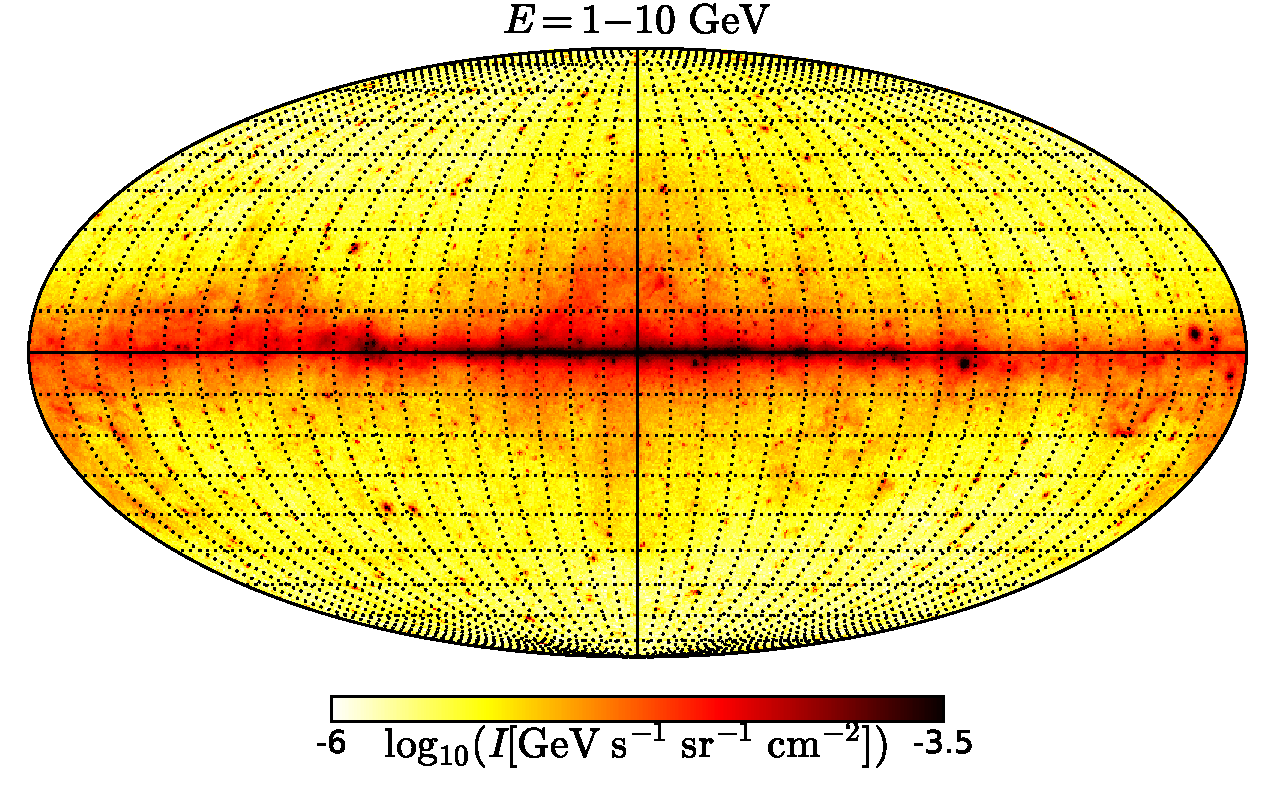
\includegraphics[width=\textwidth]{plots/Mollweide_data_source_range_0.pdf}
    	\end{subfigure} 
    	\begin{subfigure}{0.3\textwidth}
        	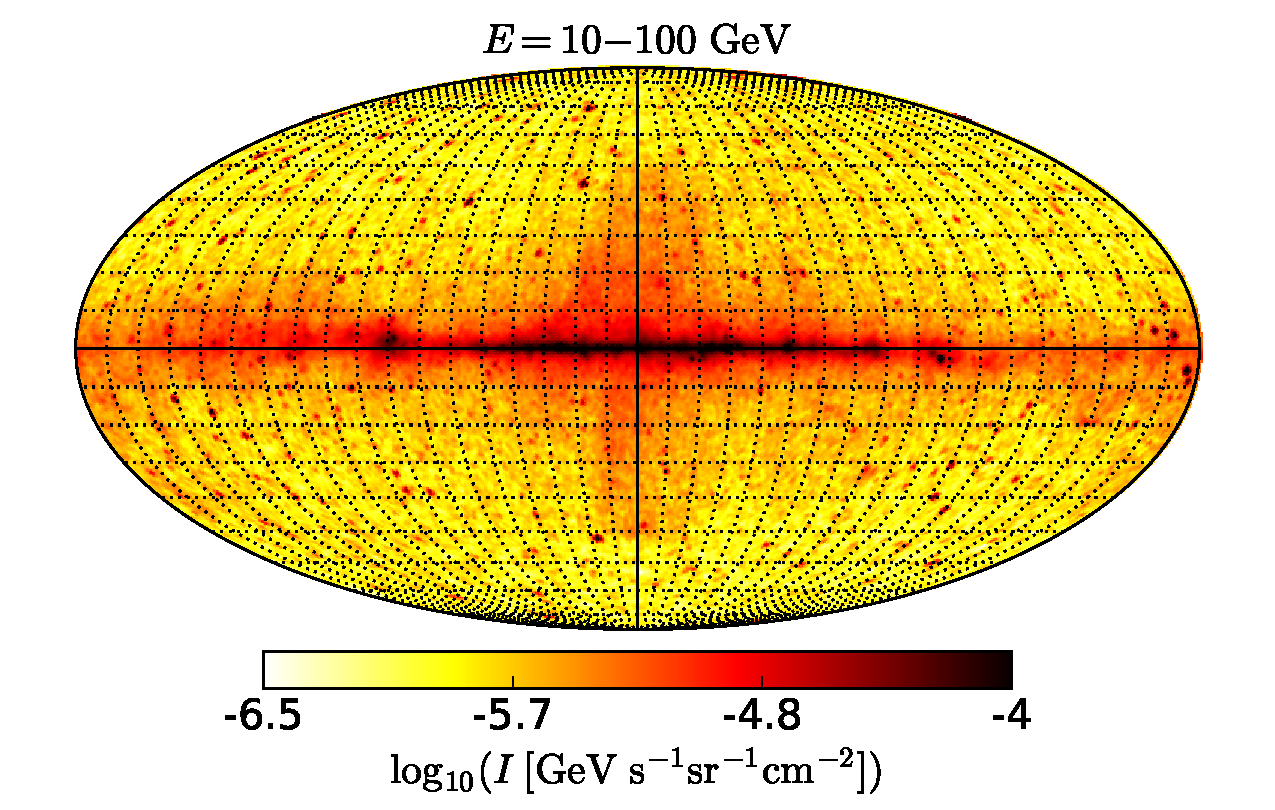
\includegraphics[width=\textwidth]{plots/Mollweide_data_source_range_1.pdf}
    	\end{subfigure}
    	\begin{subfigure}{0.3\textwidth}
        	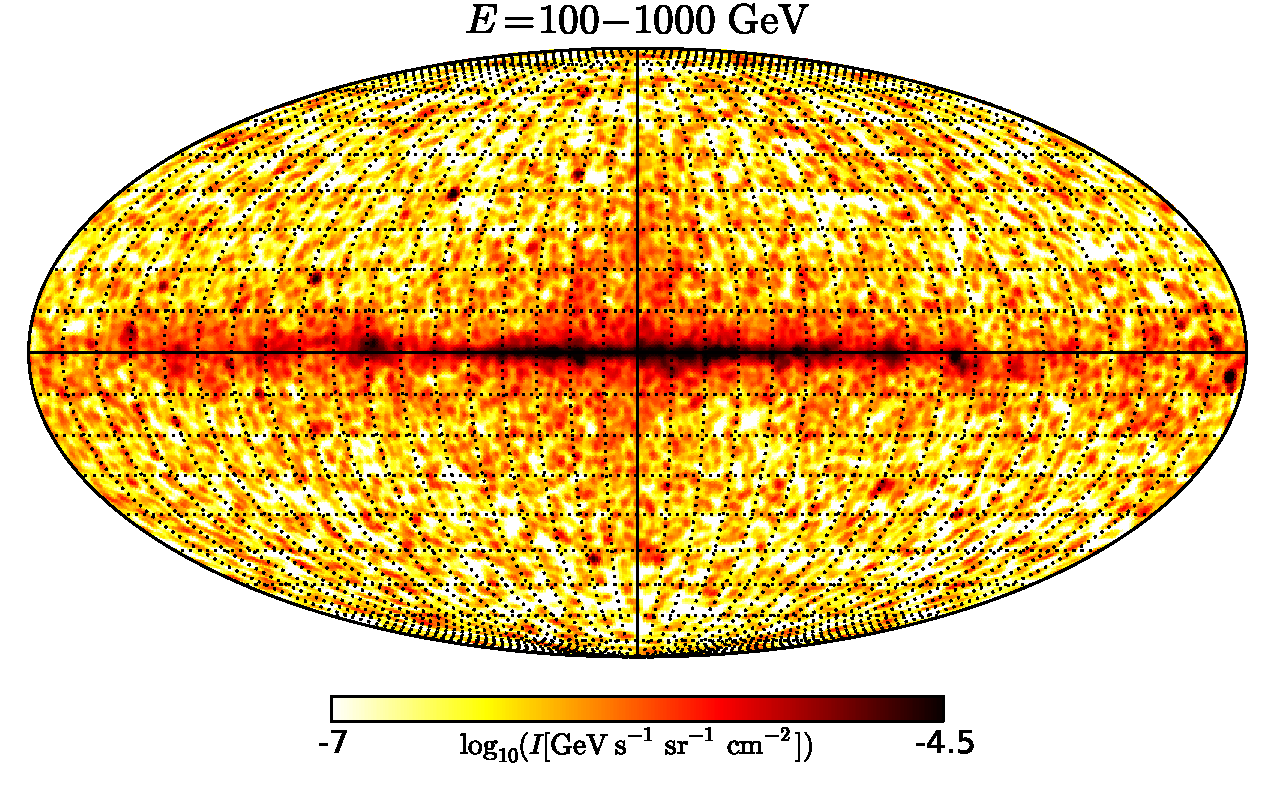
\includegraphics[width=\textwidth]{plots/Mollweide_data_source_range_2.pdf}
    	\end{subfigure}
    }
  	\caption{SED intensity integrated in three different energy ranges of the \Fermi-LAT 9 years of Source class data.}
  	\label{fig:Maps_data}
\end{figure*}

The main goal of the analysis is a study of a relatively small region $\lesssim 10^\circ$ from the GC for energies $\gtrsim 1$ GeV.
We use 9 years of the \Fermi-LAT Pass 8 Source class events
between August 4, 2008  and August 3, 2017 ({\Fermi} Mission Elapsed Time 239557418\,s -- 523411376\,s)
with energies between 316 MeV $ = 10^{2.5}$ MeV
and 1 TeV separated in 21 logarithmic energy bins (6 bins per decade).
The selection of the events is performed with the standard quality cuts.
In order to avoid contamination from gamma rays produced in interactions of cosmic ray in the Earth atmosphere, 
we select events with the zenith angles $\theta < 100^{\circ}$,
which is sufficient for energies above 316 MeV.
We calculate the exposure and point-spread function (PSF) using the {\Fermi}-LAT Science Tools package version 
10-01-01 available from the {\Fermi} Science Support Center\footnote{\url{http://fermi.gsfc.nasa.gov/ssc/data/analysis/}} 
with the P8R2\_SOURCE\_V6 instrument response functions.
Figure \ref{fig:Maps_data} shows the data in units of integrated flux in three energy ranges. For all maps shown in this paper, we use Galactic coordinates centered on the GC in Mollweide projection. The graticule spacing is $\ang{10}$ in latitude and longitude. The maps are smoothed with a $\sigma = \ang{0.5}$ Gaussian kernel.
For spatial binning we use HEALPix\footnote{\url{http://sourceforge.net/projects/healpix/}} \citep{2005ApJ...622..759G} scheme with a pixelization of order 7  ($\approx 0\degr\!\!.46$ pixel size). 


\section{Modeling of the \Fermi bubbles at low latitudes}
\label{sec:Modeling}

\begin{comment}
One of the main problems in the analysis of the FBs near the GC is the 
presence of the foreground emission components, 
such as the interactions of cosmic rays with the interstellar gas and radiation fields.
In order to test the possible effects of the foreground emission modeling,
we use several methods to estimate the contribution of the foreground emission to the data.

In particular, there is a tentative
displacement of the FBs to the right of the GC, i.e., negative Galactic latitudes \citep{2016ApJS..223...26A, 2017ApJ...840...43A},
with a spectrum that is harder than the spectrum of the FBs at high latitudes \citep{2017ApJ...840...43A}.
If we assume that the Galactic emission components are approximately symmetric with respect to the GC,
then we can simply mask PS and calculate the difference in gamma-ray flux to the left and to the right from the GC.
The difference should be approximately equal to the asymmetric part of the FBs emission
under the assumption that the other Galactic components and unresolved PS are symmetric with respect to the GC
(Section \ref{sec:data_diff}).

In order to further test the hypothesis of the asymmetric and hard emission from the FBs at low latitudes,
we use the data at energies $\lesssim \SI{1}{GeV}$ to create a template of the Galactic emission,
provided that the expected contribution of the FBs at these energies is small relative to the rest of the Galactic components.
Then we fit the template derived from the low-energy data together with an isotropic template at higher energies
outside of the FBs area.
The FBs intensity is determined by extrapolating the model inside the FBs area using the full template and by subtracting the model
from the data (Section \ref{sec:le_data_model}).
As an alternative approach, instead of fitting outside of the FBs area, we add to the model independent flat rectangular templates with the size
approximately following the FBs size and fit the model over the whole sky.
The flux attributed to these rectangular templates is used as an estimate of the average flux in the FBs in the corresponding areas
(Section \ref{sec:box_model}).

We also calculate the flux attributed to the bubbles using one of the diffuse emission models from \citep{2017ApJ...840...43A}
(Section \ref{sec:galprop_model}).

\end{comment}

\subsection{East-west  asymmetry in the data}
\label{sec:data_diff}

In order to investigate the asymmetry of the emission at the base of the FBs relative to the GC, 
we compare the \Fermi-LAT data east and west of the GC. 
We mask the 200 point sources (PS) in the Third \Fermi-LAT source catalog \citep[3FGL,][]{2015ApJS..218...23A}
with the largest flux above 1 GeV.
Each PS is masked with a circle of radius $\frac{\delta}{\sqrt{2}} + 0^\circ\!\!.5$, where $\delta = 0\degr\!\!.46$ is the characteristic size of the pixels
so that ${\delta}/{\sqrt{2}}$ is half of the pixel diagonal (if it were a square), while $0\degr\!\!.5$ is comparable to 
the 68\% containment radius of the point-spread function above $\approx 2$ GeV.
Thus the total radius is about $0\degr\!\!.82$.
In order to avoid possible bias by masking more pixels on one side of the GC in the Galactic plane,
we symmetrize the PS mask relative to the GC, i.e., we set $m_{-b, -\ell} = 0$ if $m_{b, \ell} = 0$ and vice versa.
This PS mask is also used in the following sections (apart from Section \ref{sec:galprop_model}).
The data are averaged over regions to the east ($0^\circ < \ell < 10^\circ$) and to the west ($-10^\circ < \ell  <  0^\circ$) 
of the GC at different latitudes. 
The regions have a latitude width of $4^\circ$. 
%$10^\circ$ for $b >|10^\circ|$ and a width of  $4^\circ$ for  $b <|10^\circ|$. 
The fraction of masked pixels is about 50\% within $|b| < 2^\circ$, about 10\% for $2^\circ < |b| < 6^\circ$, and less than  5\% 
for $|b| > 6^\circ$.

The difference of the averaged intensity of emission west minus east of the GC is shown in Fig. \ref{fig:data_diff}. 
The error bars represent the statistical errors.
%At high latitudes, $|b| > 10^\circ$, the emission is relatively symmetric, 
%apart from the cocoon inside the southern lobe of the FBs \citep{2012ApJ...753...61S, 2014ApJ...793...64A}.
The emission for latitudes $b \in (-6^\circ, -2^\circ)$ and $b \in (-2^\circ, 2^\circ)$ shows excess emission to the west of the GC, 
which remains significant at high energies. 
The Fermi-LAT exposure within $|b| < 10^\circ$ and $|\ell| < 10^\circ$ is rather uniform; 
the maximal fractional variation of the exposure in this region for $E > 1$ GeV is less than 4\%.

\begin{figure}[h]
%\centering
\hspace{-2mm}
 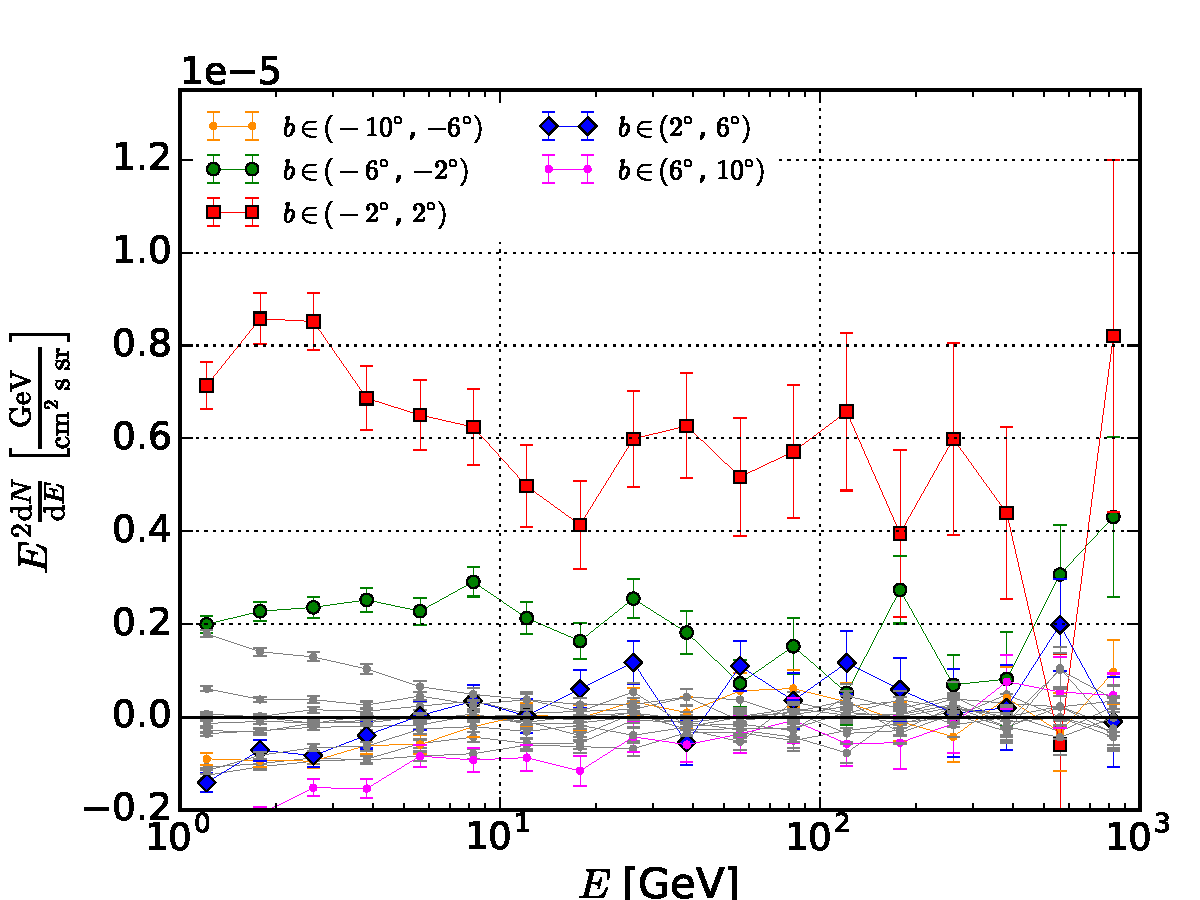
\includegraphics[width=\onepic\textwidth]{plots/Difference_data_for_different_latitudes.pdf}
 \caption{Difference west minus east in the \Fermi-LAT intensity relative to the GC after masking bright PSs.
 The PS mask is symmetrized relative to the GC.
 The west (east) region is defined between $-10^\circ < \ell <0^\circ$ ($0^\circ < \ell <10^\circ$).
 Grey lines show spectra for latitudes $|b| > 10^\circ$. 
 }
 \label{fig:data_diff}
\end{figure}

\subsection{Low-energy data as a background model}
\label{sec:le_data_model}

\begin{figure*}[t]
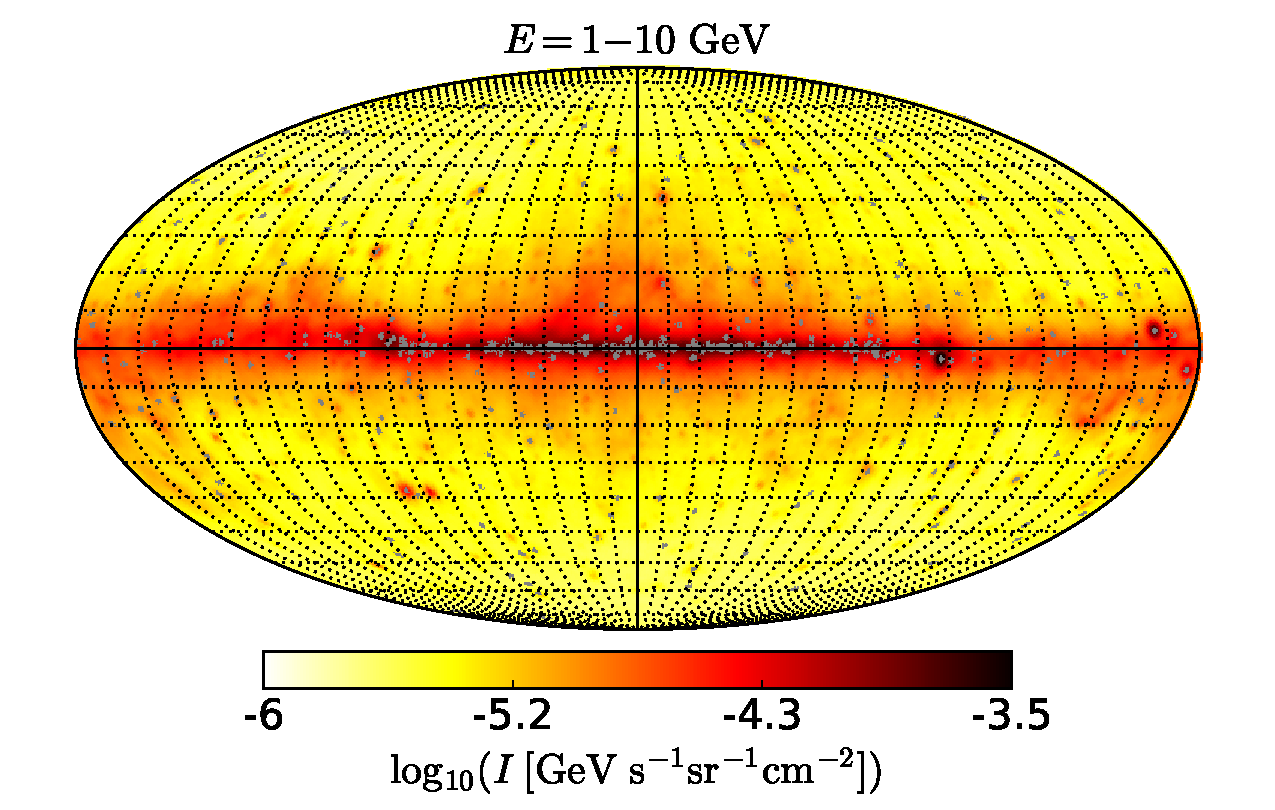
\includegraphics[width=\threepic\textwidth]{plots/Mollweide_LowE_model_0p3-1p0GeV_flux_source_range_0_log.pdf}
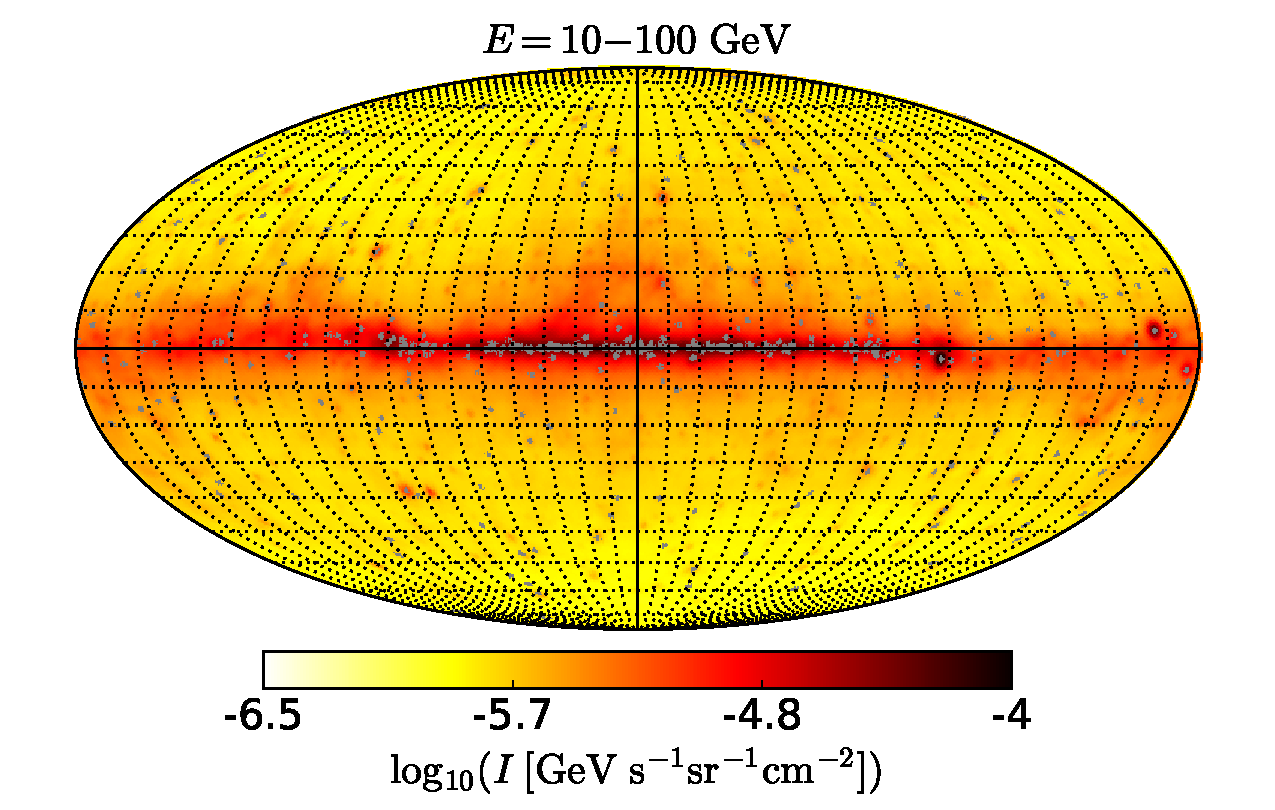
\includegraphics[width=\threepic\textwidth]{plots/Mollweide_LowE_model_0p3-1p0GeV_flux_source_range_1_log.pdf}
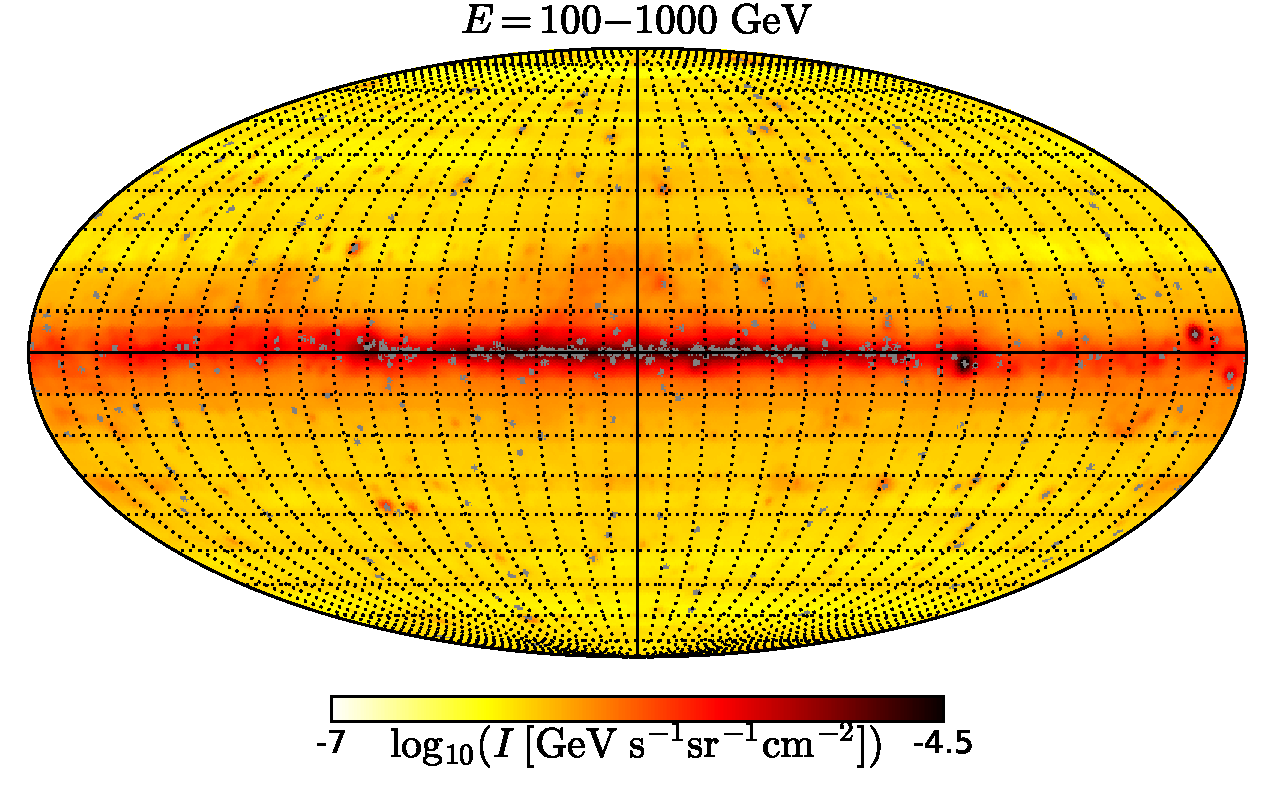
\includegraphics[width=\threepic\textwidth]{plots/Mollweide_LowE_model_0p3-1p0GeV_flux_source_range_2_log.pdf}
\caption{Energy flux of the diffuse emission model based on the low-energy data (Section \ref{sec:le_data_model})
integrated over three energy ranges. }
\label{fig:Maps_lowE_model}
\end{figure*}


\begin{figure*}[t]
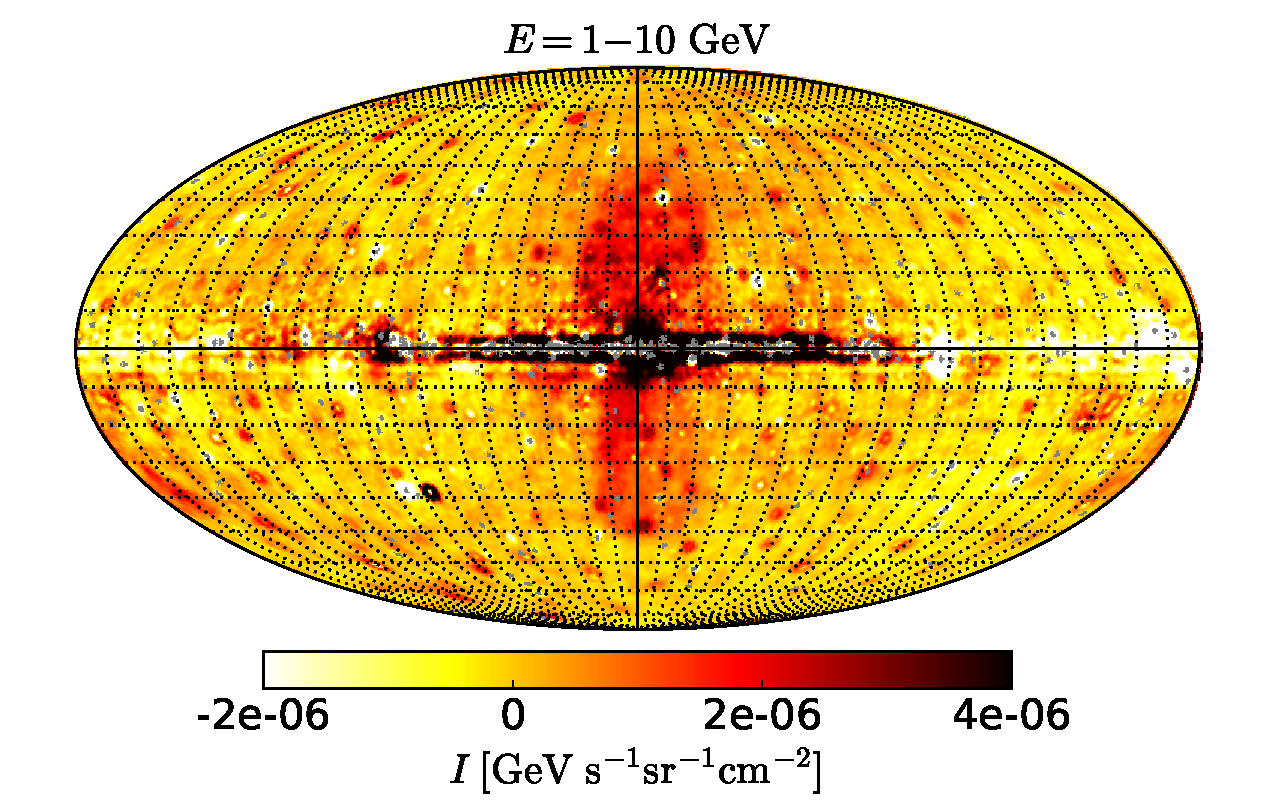
\includegraphics[width=\threepic\textwidth]{plots/Mollweide_LowE_0p3-1p0GeV_flux_source_range_0.pdf}
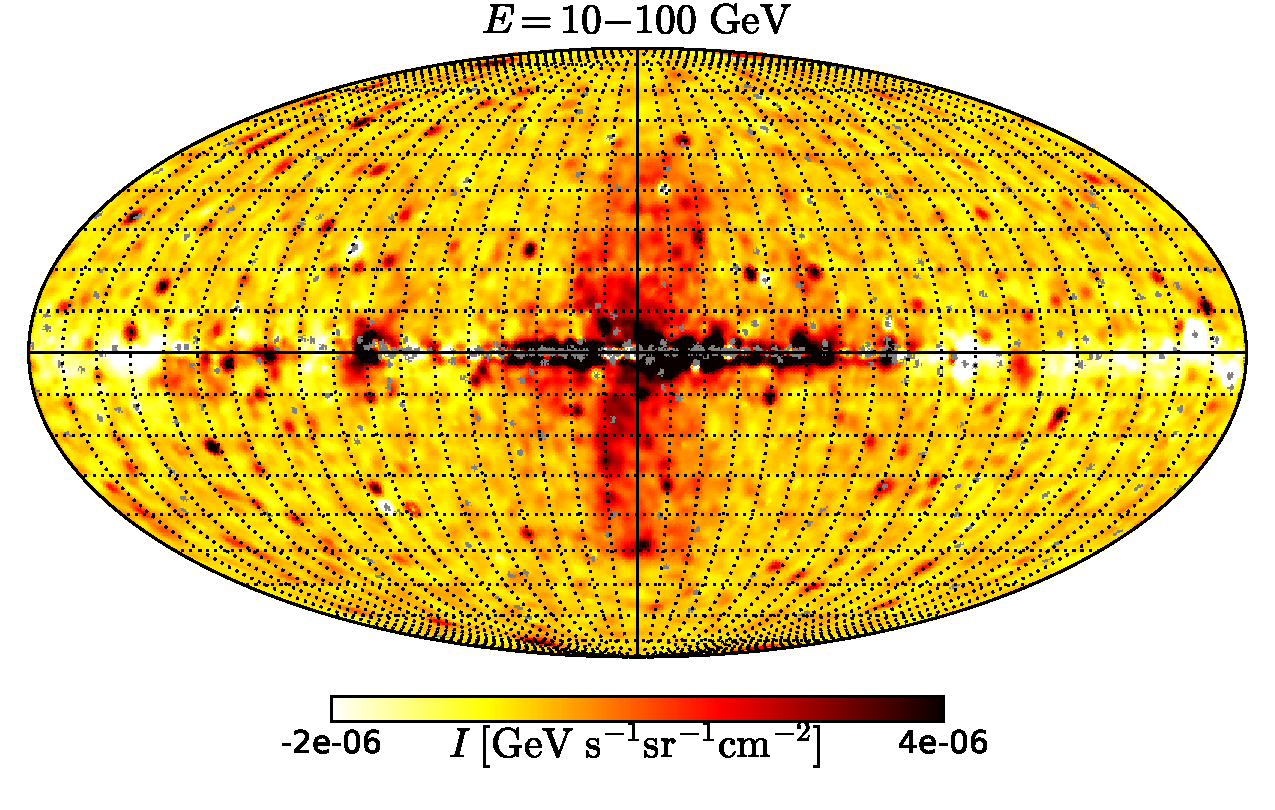
\includegraphics[width=\threepic\textwidth]{plots/Mollweide_LowE_0p3-1p0GeV_flux_source_range_1.pdf}
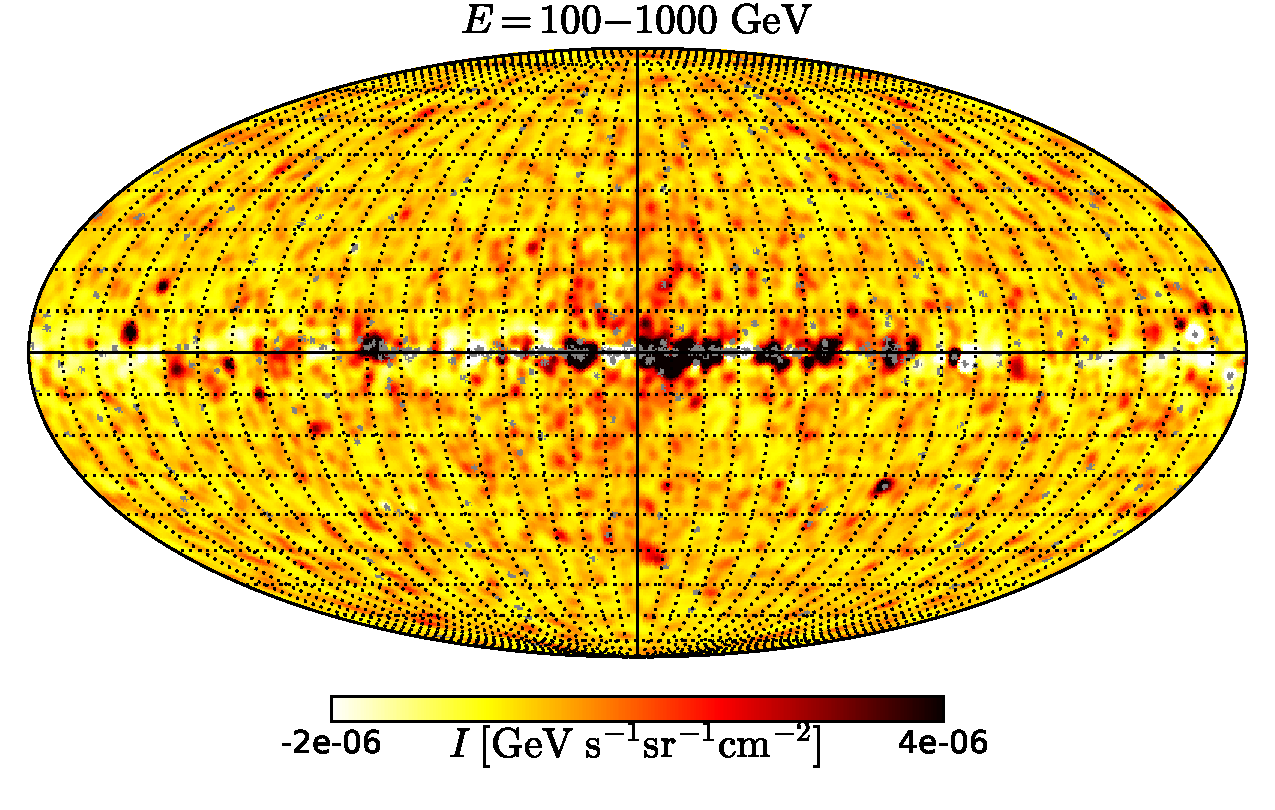
\includegraphics[width=\threepic\textwidth]{plots/Mollweide_LowE_0p3-1p0GeV_flux_source_range_2.pdf}
\caption{Energy flux of the residuals of the low-energy model derived in Section \ref{sec:le_data_model}
integrated over three energy ranges. }
\label{fig:Maps_lowE}
\end{figure*}


In the previous section we have shown that the west-minus-east difference in the \Fermi-LAT data in the Galactic plane relative to the GC has a hard 
spectrum $\sim E^{-2}$ up to 1 TeV.
One of the simplest ways to separate the soft component of emission from the hard one is to use the low-energy data as
a model of the soft component and subtract it from the data at higher energies.
Gamma rays produced in interactions of the steady state Galactic population of CR with gas and ISRF,
i.e., the $\pi^0$, bremsstrahlung, and IC components,
dominate the gamma-ray emission in the Galactic plane in the energy range $E \lesssim \SI{1}{GeV}$. 
Consequently, the low-energy \Fermi-LAT data is a good tracer for the soft components of the
diffuse gamma-ray emission in the Galactic plane and can be used to create a spatial template for the Galactic foreground.
The 68\% containment for the \Fermi-LAT photons between $\SI{316}{MeV}$ and $\SI{1}{GeV}$ (averaged with an $E^{-2}$ spectrum) is about $1^\circ\!\!.5$,
which is much larger than the sub-degree angular resolution above $\SI{1}{GeV}$.
In order to compensate for the difference in the angular resolution, 
we smooth the data in each high-energy bin above 1 GeV
with a Gaussian kernel of $\sigma = \ang{1}$ (which corresponds to $68\%$ containment angle of
$1^\circ\!\!.5$ in 2 dimensions).%
\footnote{In general, the width of the Gaussian kernel $\sigma$ can be obtained by subtracting in quadrature
the equivalent widths at low and at high energies $\sigma^2 = \sigma_{\rm low}^2 - \sigma_{\rm high}^2$.
Since $\sigma_{\rm low}^2 \gg \sigma_{\rm high}^2$, we neglect $\sigma_{\rm high}^2$ and smooth the 
data at high energies with $\sigma_{\rm low} = 1^\circ$.}

We separate the whole sky in latitude stripes of $\ang{4}$ width where the \Healpix pixels are assigned to stripes that contain the centers of the pixels.
We parametrize the model in each stripe and each energy bin independently, i.e., 
in the latitude stripe $b$ for energy bin $E$ and \Healpix pixel with index $i$ the model consists of two terms:

\be
\lb{eq:le_model}
M_{b}(E, i) = k_{b}(E) \cdot \tilde N^\low_{b}(E, i) + c_b(E) \cdot \tau(E, i),
\ee
where $k_{b}(E)$ and $c_b(E)$ are coefficients to be determined from the fit to the data.
The term $c_b(E) \cdot \tau(E, i)$ is proportional to the exposure $\tau(E, i)$: it accounts for the isotropic extragalactic background and partially compensates for 
the latitude-dependent IC emission.
$k_{b}(E) \cdot \tilde N^\low_b(E, i)$ is proportional to the low-energy photon counts summed over 
$n_\low = 3$ energy bins between $\SI{316}{MeV}$ and $\SI{1}{GeV}$ 
rescaled by the ratio of exposures at low and at high energies:

\be
\tilde N^\low_b(E, i) = \frac{1}{n_\low} \left(\sum_{\alpha = 1}^{n_\low} \frac{N(E_\al, i)}{\tau(E_\al, i)} \right)\tau(E, i),
\ee
where $N(E_\al, i)$ is the number of photons in energy bin $E_\al$ and in pixel $i$.

We determine the parameters $c_{b}(E)$ and $k_{b}(E)$ by fitting the model to the \Fermi-LAT data in energy bins 
$E > \SI{1}{GeV}$.
We maximize the log likelihood of the gamma distribution 
with respect to parameters $c_{b}(E)$ and $k_{b}(E)$
using the Python iminuit optimizer%
\footnote{
The gamma distribution $p(x; \td{k} + 1) = \frac{x^{\td{k}}}{\G (\td{k} + 1)}e^{-x}$ is the probability density function
for the parameter $x$ given the observed counts $\td{k}$.
The counts $\td{k}$ are integer for unsmoothed maps and non-integer for the smoothed maps.
We discuss the optimization of the model parameters using smoothed maps in 
Appendix \ref{app:gamma}.
}.
In order to avoid an overcompensation 
for the flux from the FBs, the region $-20^\circ < \ell < 20^\circ$
is excluded from the fit, i.e., the fit is performed for 
the total remaining length of the stripe $20^\circ < \ell < 340^\circ$.
In the following, the region $-20^\circ < \ell < 20^\circ$ will be refered to as the FBs region of interest (ROI).
Bright PSs are masked with the mask described in Section \ref{sec:data_diff}.

%\red{Dima: do we symmetrize the PS mask in the analysis as well, not only in the calculation of the asymmetry in the data?}

After we fit the model in each latitude stripe, we interpolate it inside the bubbles ROI.
The intensity of the model energy flux integrated in three energy ranges
is shown in Figure \ref{fig:Maps_lowE_model},
while the residuals after subtracting the model from the data are presented in Figure \ref{fig:Maps_lowE}.
The FBs are clearly visible in the first two energy ranges, $E = 1 - \SI{10}{GeV}$ and $E = 10 - \SI{100}{GeV}$.
For $E = \SI{100}{GeV} - \SI{1}{TeV}$ the statistics are low, but one can still see an excess near the GP.
There are other regions of large residuals in the Galactic plane as well as at high latitudes.
These are diffuse and point-like sources with spectra harder than the average spectra of Galactic and
extragalactic sources.
In particular, there is a residual in diffuse emission along the Galactic plane within $|\ell | \lesssim 60^\circ$ at energies below 100 GeV.
This residual can be due to IC emission, which has a harder spectrum than the average spectrum of the $\pi^0$ component,
or to a harder spectrum of cosmic rays in the inner Galaxy \citep{2015PhRvD..91h3012G, 2016ApJS..223...26A},
or to a population of hard PSs in the Galactic plane in the inner parts of the Galaxy.
At energies above 100 GeV the residuals are resolved into localized sources, some of which are extended.
Apart from the Galactic foreground and background components, there are gamma rays emitted by the interactions of CRs with 
the Sun and its radiation field \citep{2011ApJ...734..116A} and the Moon \citep{2016PhRvD..93h2001A}.
The intensities of the emission from the Sun and the Moon are about an order of magnitude less than 
the intensity of the emission from the FBs. 
As a result, these components are not visible on  the residual maps at energies above 10 GeV.

%\newpage

\subsection{Rectangles model of the bubbles}
\label{sec:box_model}

In the previous subsection, we exclude the ROI of the FBs.
In this subsection, we perform the fit over the whole sky and model the emission from the FBs using rectangles.
%Our first simple ansatz for a model of the FBs consists of rectangular templates that approximately cover the area of the FBs. 
In order to explore the east-west asymmetry of the FBs, 
we introduce two rectangular templates in each latitude stripe $b$ and energy bin $E$: 
one east, $\ell \in (-20^\circ, 0^\circ)$, and one west, $\ell \in (0^\circ, 20^\circ)$, of the GC.
The width of the rectangles is $4^\circ$, i.e., the same as the width of the latitude stripes.
%Below $|b| = 10^\circ$, the width of the rectangles is $4^\circ$ with centers at $b = 0^\circ,  \pm 4^\circ,  \pm 8^\circ$,
%while above $|b| = 10^\circ$ the width is $10^\circ$ with centers at $b = \pm 15^\circ,  \pm 25^\circ,  \ldots, \pm 55^\circ$.
We use the same foreground model as in Section \ref{sec:le_data_model} plus the isotropic template.
Overall, the model has four terms in each energy bin:

\be
\begin{split}
M_{b}(E, i) &= k_{b}(E) \cdot \tilde N^\low_{b}(E, i) + c_b(E) \cdot \tau(E, i)\\
& + R^\east_b(E) S^\east_b(i)+ R^\west_b(E) S^\west_b(i).
\end{split}
\ee
where the scaling parameters $k_{b}(E)$ and $c_{b}(E)$
and the FBs model parameters $R^\east_b(E)$ and $R^\west_b(E)$ are determined independently 
in each $4^\circ$ latitude stripe and in each energy bin $E > 1$ GeV
by fitting the model to the smoothed \Fermi-LAT data
(see Section  \ref{sec:le_data_model} for details on the smoothing of the data).
$S_b^\east(i)$  and $S_b^\west(i)$ are step function templates, which are equal to 1 in each latitude stripe $b$
for $0^\circ < \ell < 20^\circ$ and $0^\circ > \ell > - 20^\circ$ respectively and 0 otherwise.
The energy fluxes of the model and the residuals integrated for $E = 10 - \SI{100}{GeV}$ are shown in Fig. \ref{fig:Maps_Rectangles}.
%Here we plot the sum of the residual and the rectangles model.
%With residual we denote the sum of the rectangles-model residual and the rectangles template in the following.

\begin{figure*}[h]
\centering
 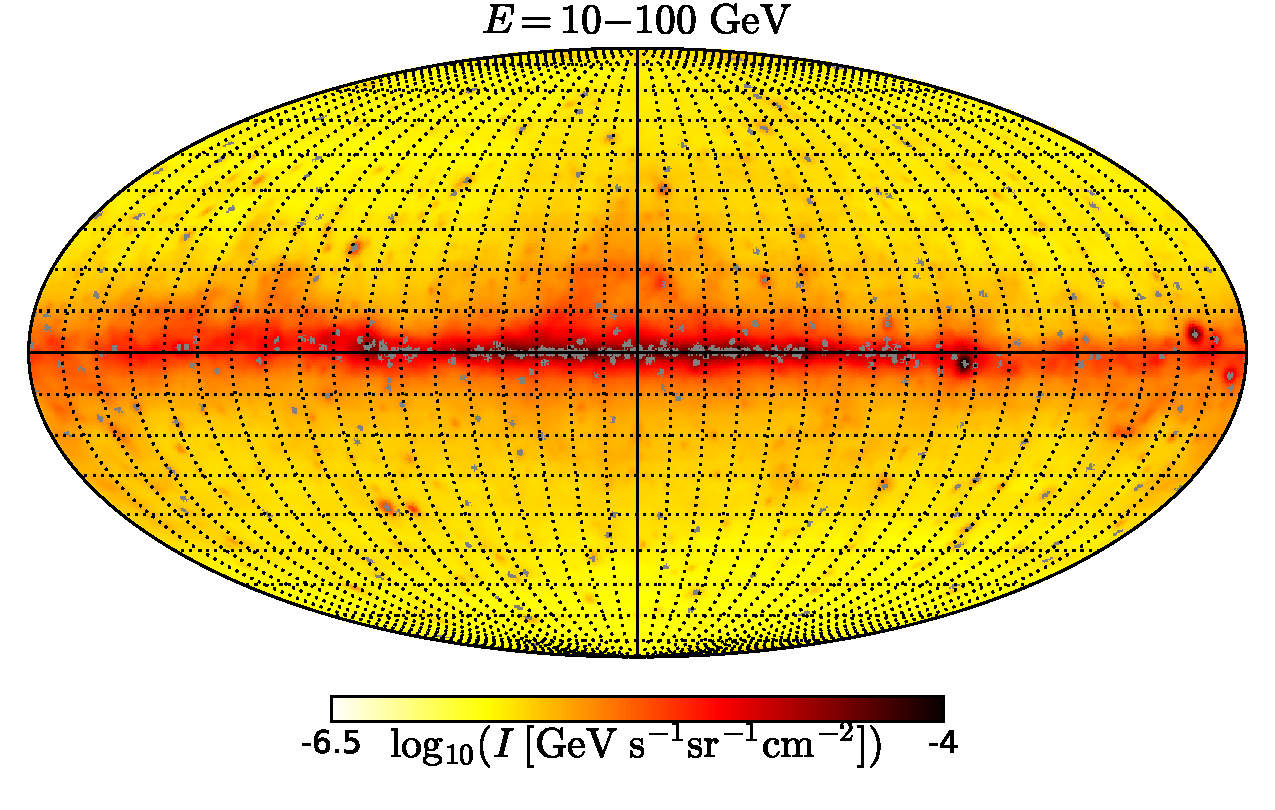
\includegraphics[width=\twopic\textwidth]{plots/Mollweide_Boxes_model_0p3-1p0GeV_flux_source_range_1_log.pdf}
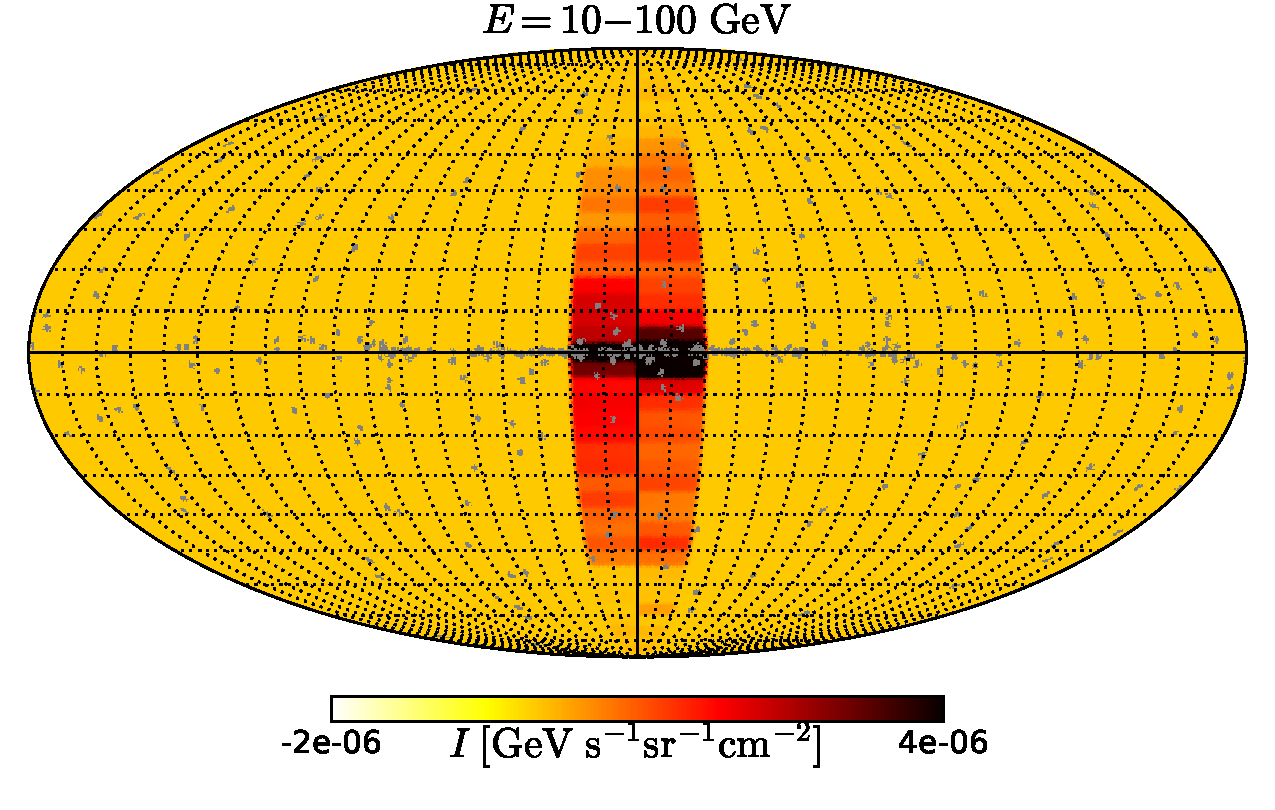
\includegraphics[width=\twopic\textwidth]{plots/Mollweide_Boxes_0p3-1p0GeV_flux_source_range_1.pdf}\\
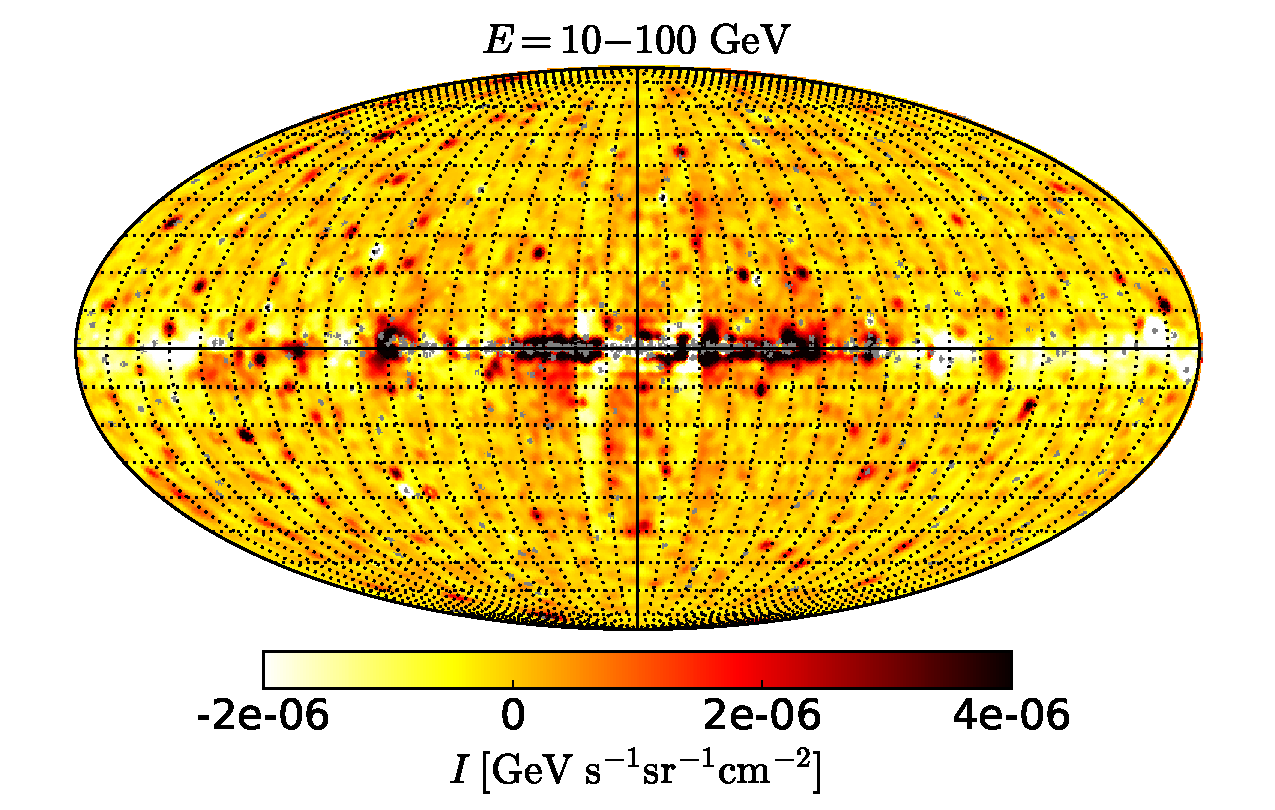
\includegraphics[width=\twopic\textwidth]{plots/Mollweide_Boxes_residual_0p3-1p0GeV_flux_source_range_1.pdf}
 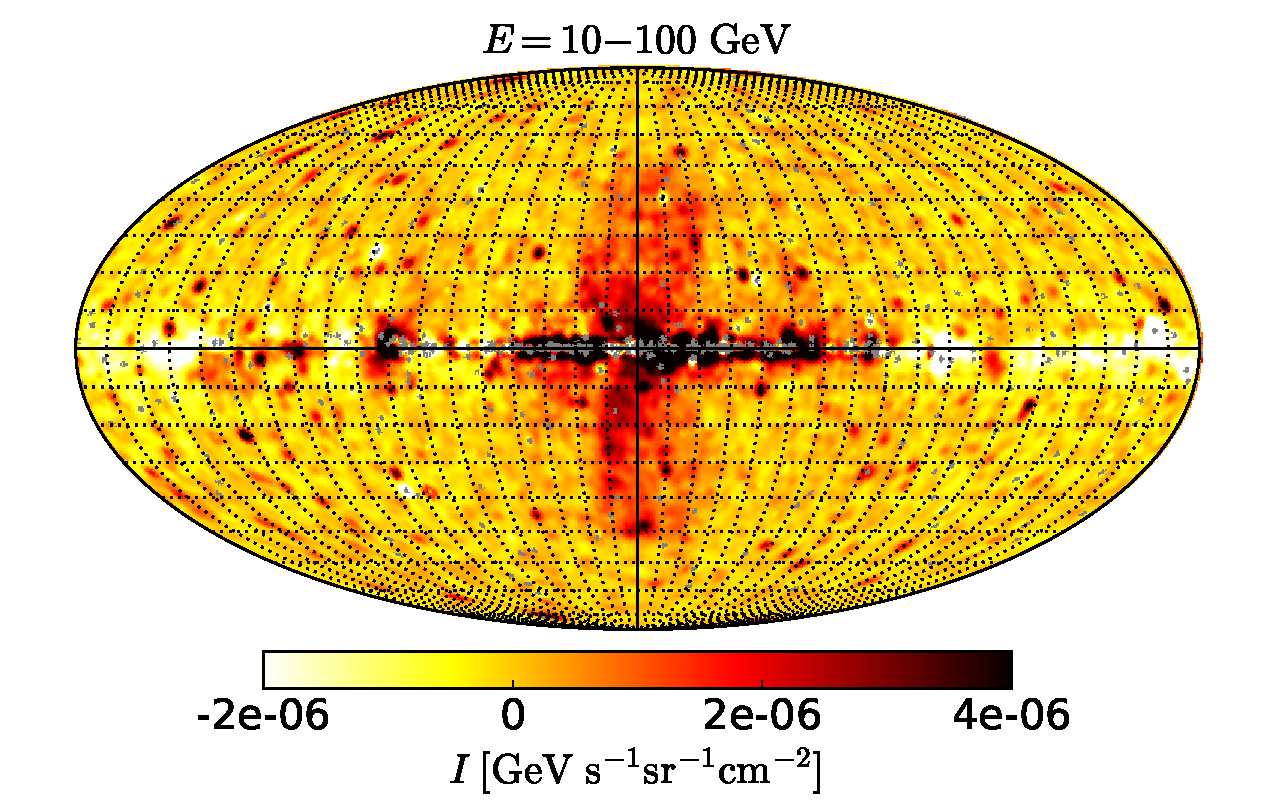
\includegraphics[width=\twopic\textwidth]{plots/Mollweide_Boxes_residual+boxes_0p3-1p0GeV_flux_source_range_1.pdf}
 \caption{Energy flux of the diffuse model excluding the rectangles model of the FBs (top left),
 the rectangles model of the FBs (top right), 
the residual after subtracting the total model (bottom left),
and residuals plus the rectangles model of the FBs (bottom right)
 derived in Section \ref{sec:box_model}
 integrated between 10 and 100 GeV.}
 \label{fig:Maps_Rectangles}
\end{figure*}

\subsection{GALPROP model of the foreground and PS refitting}
\label{sec:galprop_model}


\begin{figure*}[h]
\centering
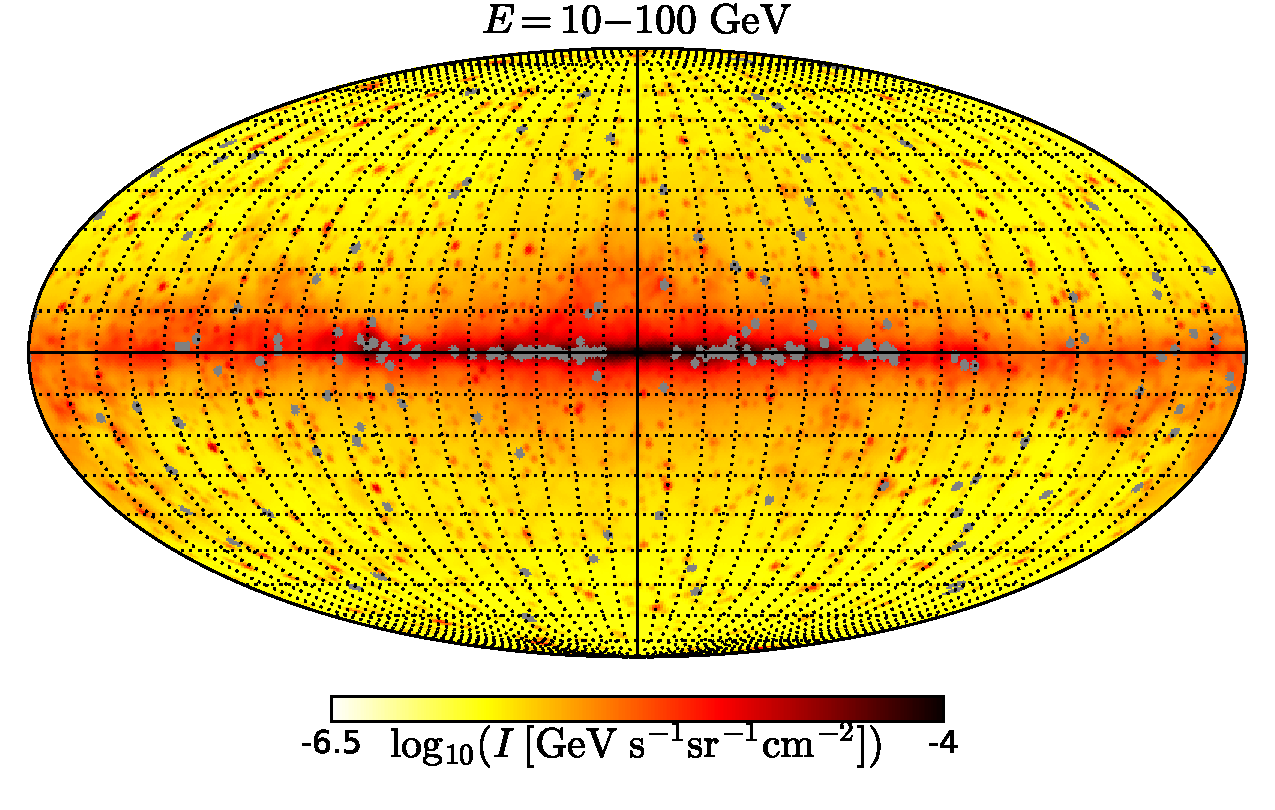
\includegraphics[width=\twopic\textwidth]{plots/Mollwiede_GALPROP_model_source_range2_log.pdf}
 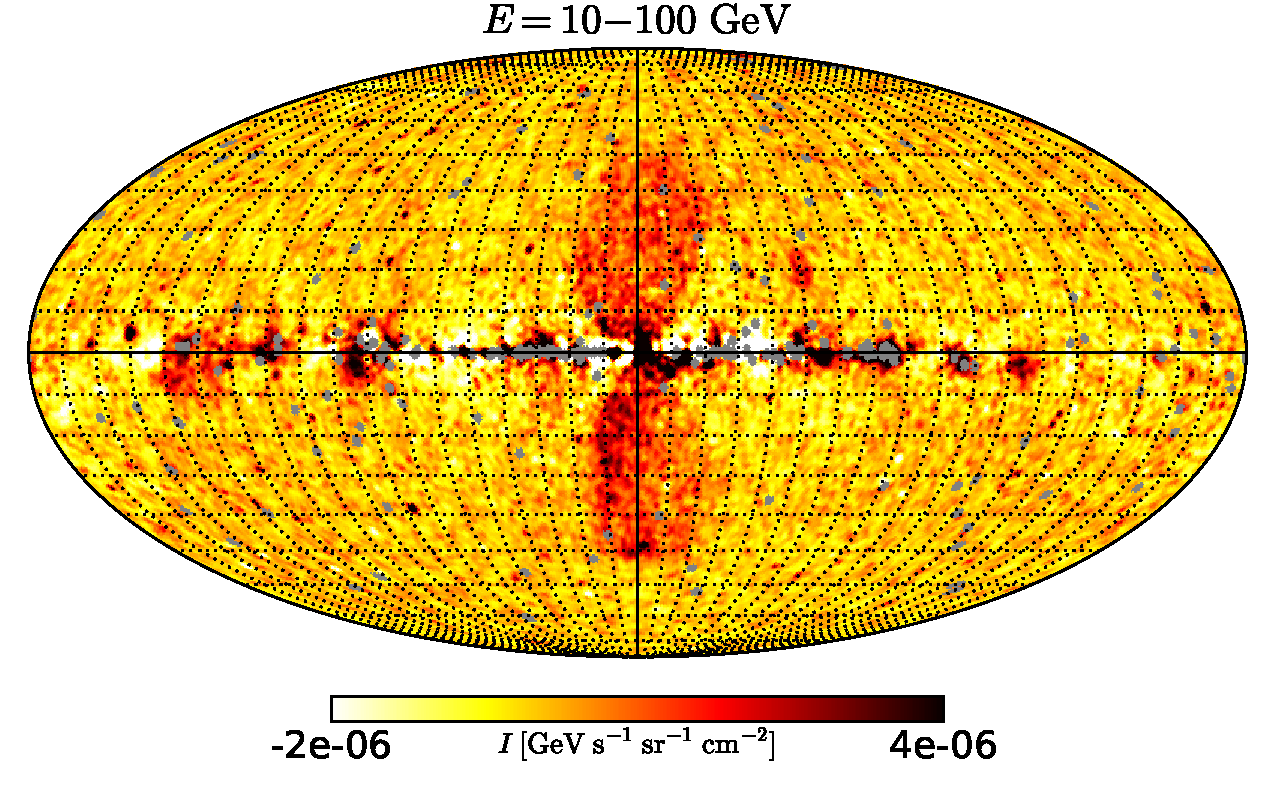
\includegraphics[width=\twopic\textwidth]{plots/Mollwiede_GALPROP_source_range2.pdf}
 \caption{Energy flux of the background model based on rescaled GALPROP templates (left)
 and of the residuals plus the FBs and the gNFW component (right) derived in Section \ref{sec:galprop_model}
 integrated between 10 and 100 GeV.}
 \label{fig:Maps_GALPROP}
\end{figure*}

In this section we fit the gamma-ray data using a model derived with the GALPROP
Galactic cosmic-ray propagation code v54.1.
%\citep{Moskalenko:1997gh, Strong:1998fr, Strong:2004de, Ptuskin:2005ax, 2007ARNPS..57..285S, Porter:2008ve,Vladimirov:2010aq}\footnote{\url{http://galprop.stanford.edu}}. 
The model for the diffuse emission components is the same as the Sample model in \cite{2017ApJ...840...43A}.
%The difference is that, within $10^\circ$ from the GC, we do not mask PS and refit 40 PS with largest flux between 10 and 100 GeV.
In particular, we use the GALPROP code to calculate templates for the Galactic diffuse emission components.
We determine 5 templates in each energy bin for gamma rays produced in 
interactions of hadronic CR with gas and bremsstrahlung emission corresponding to 5 Galactocentric rings: 
0 -- 1.5\,kpc, 1.5 -- 3.5\,kpc, and 3.5 -- 8\,kpc; 8 -- 10\,kpc, and 10 -- 50\,kpc.
We assume propagation halo height of 10 kpc and radius of 20 kpc and spin temperature 150 K.
We use 3 inverse Compton templates corresponding to the three ISRF: CMB, 
infrared emission of dust, and starlight.
In addition to GALPROP templates, we use a flat template for the \Fermi bubbles at latitudes $|b| > 10^\circ$~\citep{2014ApJ...793...64A}. 
We model the Loop~I feature using a geometric template \citep[e.g., Figure 2 of][]{2014ApJ...793...64A}
based on a polarization survey at 1.4 GHz~\citep{Wolleben:2007pq}.
Templates for the gamma-ray emission from the Sun  and the Moon
\citep{2008A&A...480..847O, 2011ApJ...734..116A, 2013arXiv1307.0197J, 2016PhRvD..93h2001A}
 %\citep{2007Ap&SS.309..359O, 2006ApJ...652L..65M}
are obtained with the \Fermi Science Tools%
\footnote{\url{http://fermi.gsfc.nasa.gov/ssc/data/analysis/scitools/solar_template.html}}.
We also include, as a GC excess template, 
DM annihilation with a generalized Navarro-Frenk-White (gNFW) profile with index $\gamma = 1.25$ 
\citep{Goodenough:2009gk,Abazajian:2014fta, Calore:2014xka}
and scaling radius $r_{\rm s} = 20\;{\rm kpc}$, as well as the isotropic template to model the non-resolved 
extragalactic sources.


For the PS, we add sources from the 3FGL catalog~\citep{2015ApJS..218...23A} to form a template
in each energy bin.
We create independent templates for the Large Magellanic cloud and the Cygnus region.
The remaining extended sources are also added in a separate template.
The spatial templates for the extended sources are provided by the 3FGL catalog.
The PS mask in this section is different from the mask that we have used in the previous sections.
We mask the 200 sources with largest flux above 1 GeV outside a $10^\circ$ circle from the GC.
Each source is masked with a circle of $\frac{\delta}{\sqrt{2}} + 1^\circ$ radius ($\delta = 0\degr\!\!.46$ is the characteristic size of the pixels),
which is larger than the radius of  $\frac{\delta}{\sqrt{2}} + 0^\circ\!\!.5$ used in the previous sections.
We do not mask PS within $10^\circ$ from the GC.
Instead, we include independent templates for 40 sources with largest flux between 10 and 100 GeV
taken from the column ``Flux10000\_100000'' in the 3FGL catalog.
Each source is fit in each energy bin independently, i.e., we do not use the spectral information from the 3FGL catalog.
In Figure \ref{fig:Maps_GALPROP} we show the residual emission plus the \Fermi bubbles model and the gNFW model summed over energies between 10 and 100 GeV.
Due to the model having more free parameters in the Galactic plane relative to the models considered in the previous sections,
there are fewer positive residuals in the Galactic plane.
There are, however, negative residuals in several locations, which indicates errors in the model. 
In particular, there is a rather significant negative residual to the east of the GC.
Nonetheless, the FBs are clearly visible as well as the bright emission at the base of the FBs which also displays a shift to negative
longitudes relative to the GC.



\section{Morphology and spectrum of the gamma-ray emission at the base of the FB}


\subsection{Latitude profiles}
\label{sec:Latitude_profiles}

In order to quantitatively estimate the difference in the intensity of emission of the FBs at high and at low latitudes, as well as the asymmetry
of the gamma-ray emission at the base of the FBs,
we plot the latitude profiles to the east and to the west of the GC.
In Figure \ref{fig:Profiles} we show the profiles of energy flux between 10 -- 100 GeV as a function 
of the Galactic latitude for different models of Galactic foreground emission.
%The regions have a width of $\ang{4}$ for $|b|<\ang{10}$ and $\ang{10}$ for $|b|>\ang{10}$ in latitude and a width of $\ang{10}$ in longitude. 
%that is $\ang{0} - \ang{10}$ to the east of the GC an $\ang{-10} - \ang{0}$ to the west of the GC. 
%The profiles of the three models include the residual emission plus the FBs, i.e. 
For the low-energy model, the profiles show the residual gamma-ray emission, 
for the rectangles model -- the sum of residual emission and the rectangles templates model, 
and for the GALPROP model --  the sum of residual emission, the FBs template, 
and the GC excess template, as described in Section \ref{sec:Modeling}. 
For comparison we show the latitude profile of the total gamma-ray data (excluding pixels in the PS mask).
%We observe an agreement between all models and a east-west assymmetry close to the GC. 
For positive longitudes,
some models overpredict the gamma-ray data near the GP which leads to negative residuals.
For negative longitudes, there is an increase of flux at the base of the FBs 
by at least a factor of 2 to 6 for all models relative to the gamma-ray emission from the FBs at high latitudes. 
The results for the GALPROP model differ from the low-energy and rectangles model in the Galactic plane by a factor of 2 to 3. 
This is due to additional freedom in the GALPROP model related to the usage of several templates in the Galactic plane.
%the inability of the GALPROP templates to fit the data is also manifested by the negative residuals to the east of the GC.
%Also the data shows a slight east-west assymmetry in the flux around the GC.


\begin{figure*}[h]
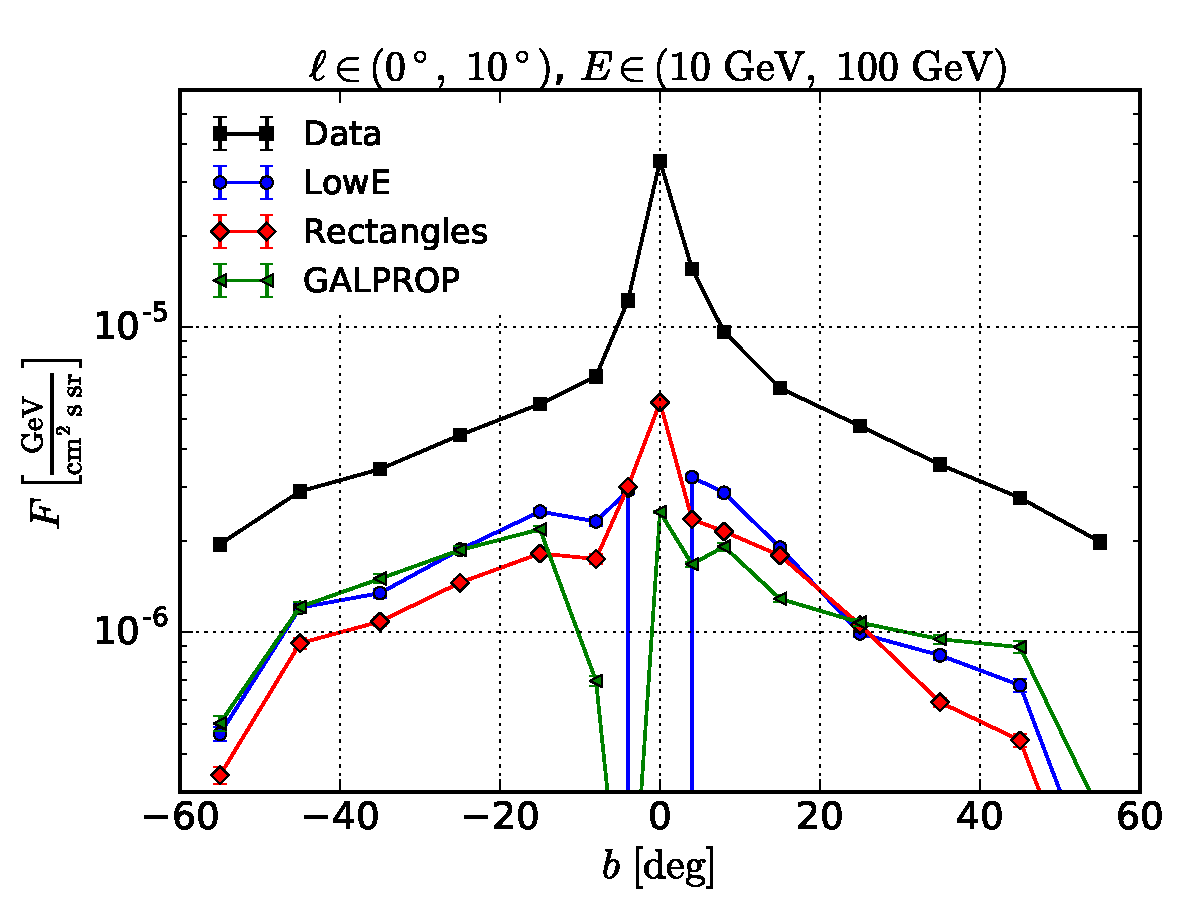
\includegraphics[width=0.5\textwidth]{plots/Profiles_l=1_source_range_1.pdf}
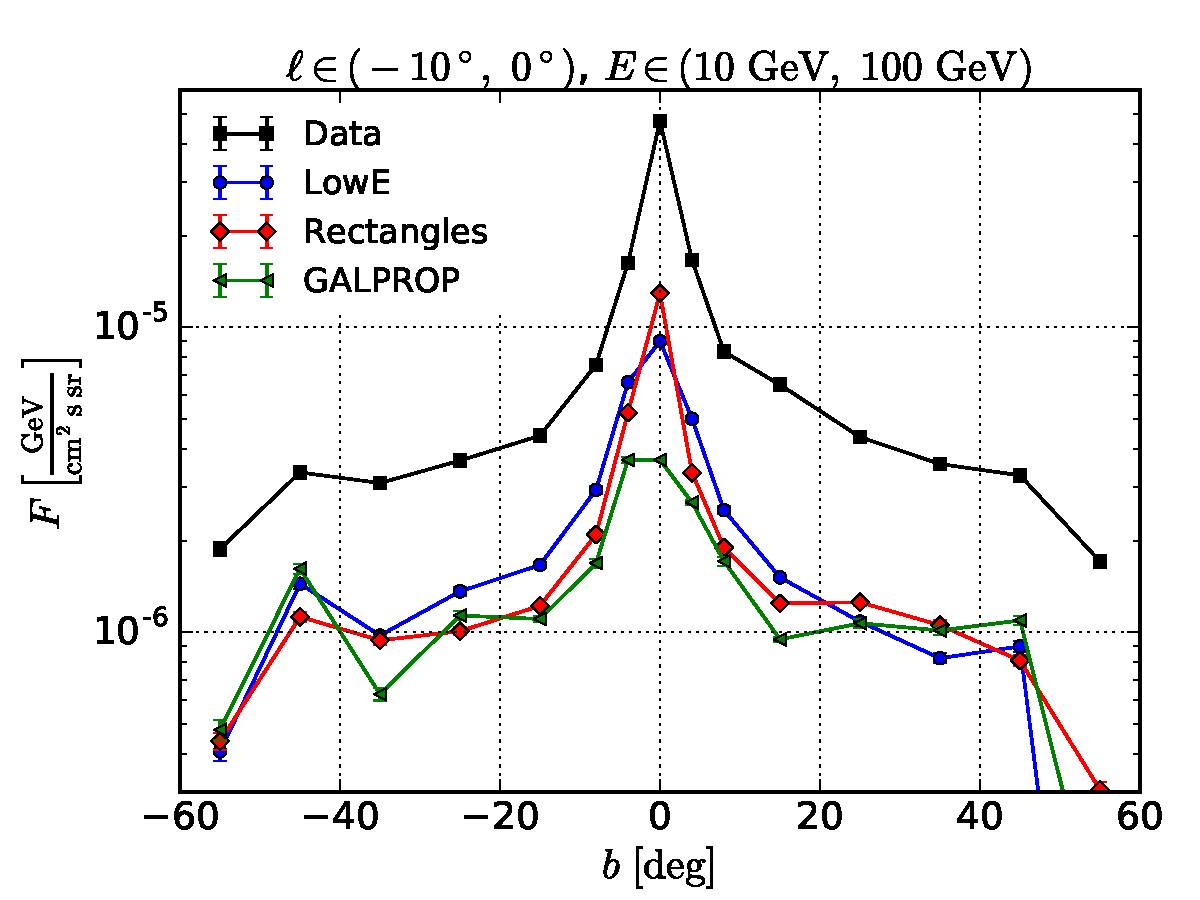
\includegraphics[width=0.5\textwidth]{plots/Profiles_l=0_source_range_1.pdf}
  	\caption{Latitude profiles of the energy flux between 10 and 100 GeV for the total data excluding the PS mask and for 
	the residuals including the FBs for 
	different diffuse emission models to the east and to the west of the GC.}
  	\label{fig:Profiles}
\end{figure*}

\subsection{Comparison of the spectra at different latitudes}

\begin{figure*}[h]
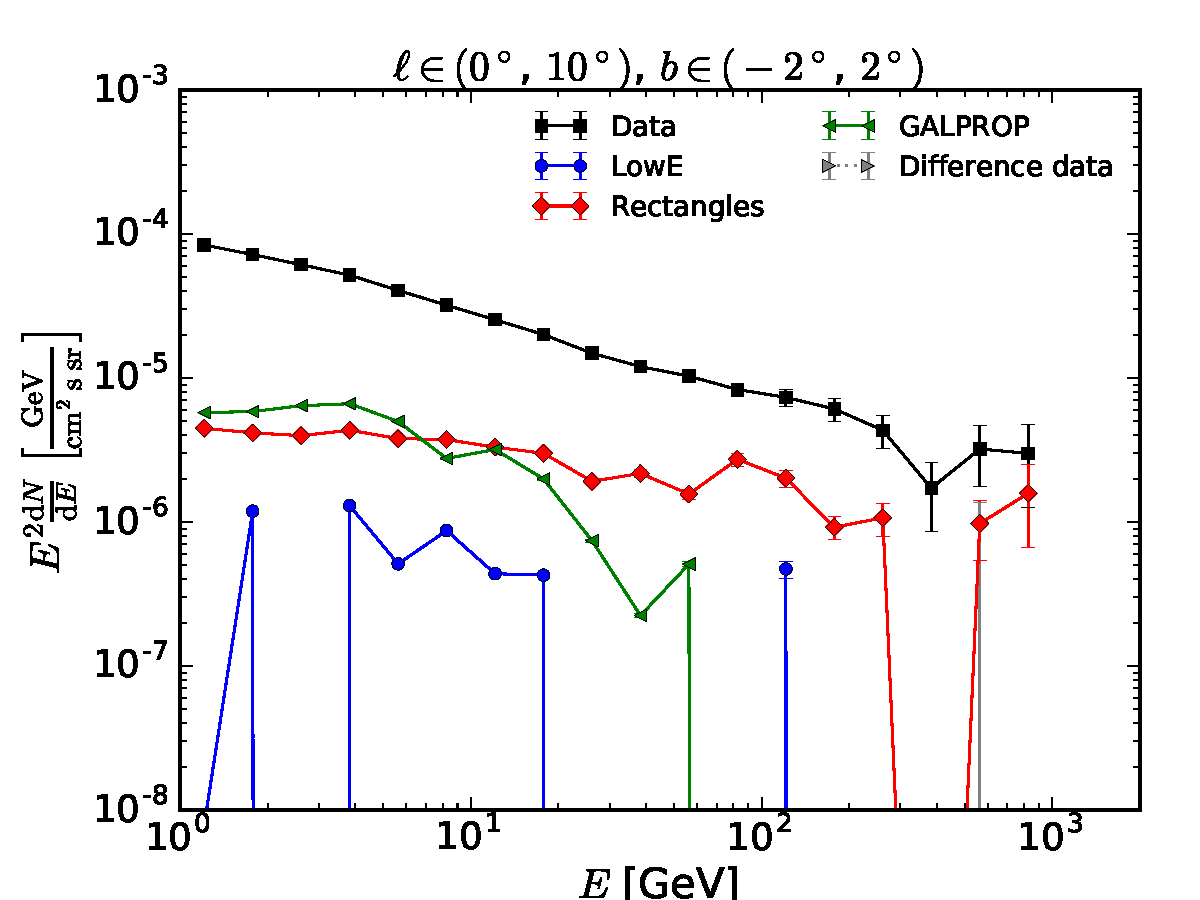
\includegraphics[width=0.5\textwidth]{plots/SED_all_models_source_l=5_b=0.pdf}
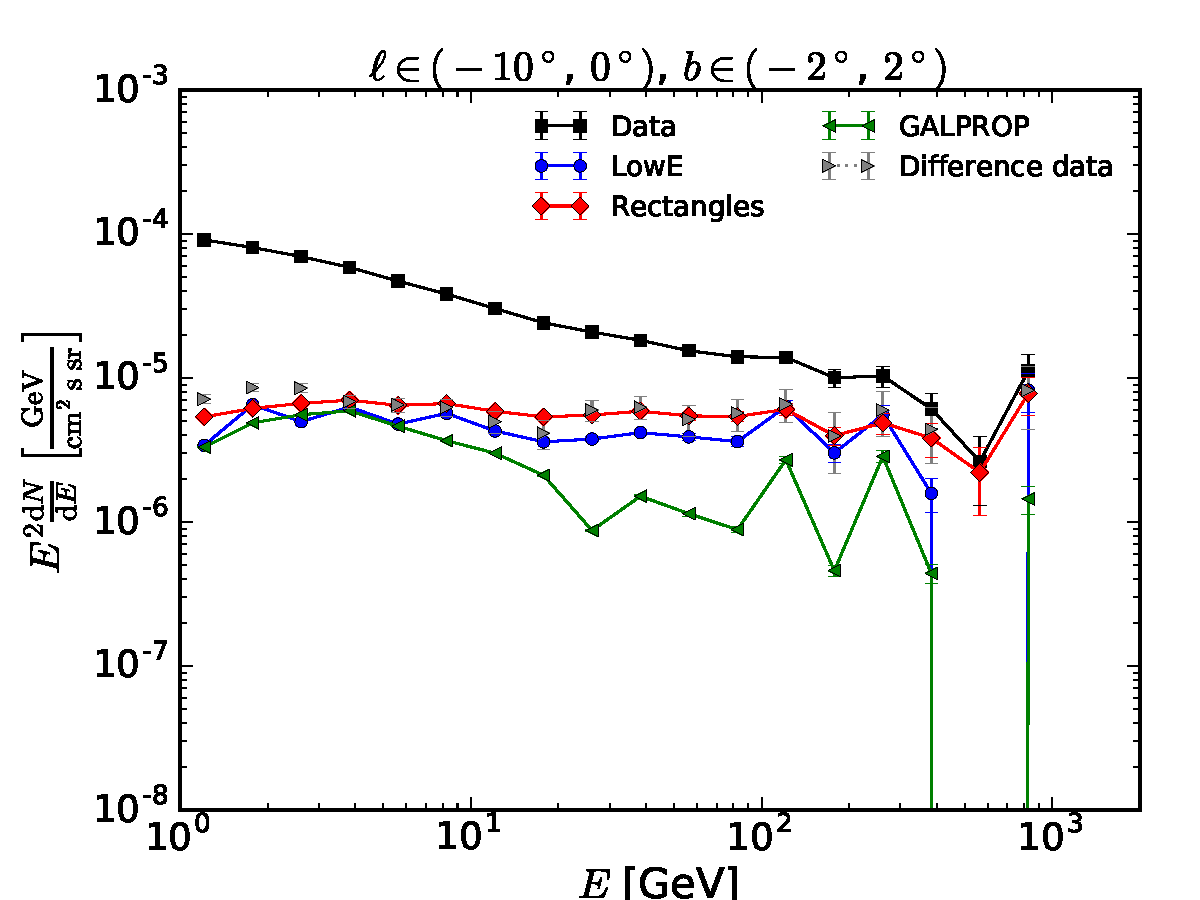
\includegraphics[width=0.5\textwidth]{plots/SED_all_models_source_l=-5_b=0.pdf}
  	\caption{SED of the residuals plus the FBs, the data, and the difference in the data west minus east of the GC (excluding pixels in the PS mask). 
	%The width of the regions in longitude is $\ang{10}$, i.e. $\ang{0}$ to $\ang{10}$ to the east of the GC (left) and $\ang{-10}$ to $\ang{0}$ to the west of the GC (right).
	}
  	\label{fig:SED_all}
\end{figure*}

In this section we quantify the hardening of the gamma-ray spectrum at the base of the FBs. 
We first compare the spectral energy distribution (SED) of the emission at the base of the FB for different foreground models in Figure \ref{fig:SED_all}. 
The differential flux is averaged over regions to the east, $\ell \in (\ang{0},\ \ang{10})$, and to the west, $\ell \in (\ang{-10},\ \ang{0})$, of the GC
in a thin stripe covering the Galactic plane $b \in (\ang{-2},\ \ang{2})$. 
For comparison, we show the total data (excluding pixels masked by the PS mask) and, on the plot for $\ell \in (\ang{-10},\ \ang{0})$, the difference in the data west minus east
of the GC.

For negative longitudes, all models give similar results. 
The differential flux of the GALPROP model is smaller than the differential flux of the other models above 10 GeV, 
which is consistent with the profile plots in Figure \ref{fig:Profiles}.
%We also find an asymmetry in the flux of the data with PS mask. 
The difference of the data west minus east of the GC is similar to the fluxes at the base of the FB in the low-energy model and in the rectangles model. 
The spectra at positive longitudes show large oversubtractions and softer indices. 
%\Laura{Should we show here the plots for (-6,-2) and (2,6) deg latitude also?}
%\dima{I'm not sure, it will take space}

To compare the behavior of the energy spectra at high energies for different latitudes, 
we fit a log-parabola plus the fixed foreground model counts to the 
total smoothed gamma-ray counts in each latitude stripe using the likelihood based on gamma distribution.
We use the following parametrization of the log-parabola function:

 \be
 f(E) = N_0 \left(\frac{E}{\SI{1}{GeV}}\right)^{-\alpha - \beta \ln(E)}.
 \ee
The local ``index'' of the spectrum at energy $E$ is

\be 
\lb{eq:log_par}
n \equiv - \frac{\de \ln f}{\de \ln E} = \alpha + 2 \beta \ln\left(\frac{E}{\SI{1}{GeV}}\right).
\ee
In Figure \ref{fig:logpar_index} we compare this log-parabola index $n$ as a function of latitude at $E = \SI{500}{GeV}$. 
%\Laura{You called it bubble! ;)} \dima{bubble removed}
We plot $(2 - n)$, which corresponds to the SED index.
For positive longitudes, the index is relatively soft ($n > 2$) for most of the latitudes
except high latitudes where the gamma-ray statistics is small.
For negative longitudes, the index near the GC
is significantly harder ($n \approx 2$) than the index at higher latitudes.
%\Laura{Would you like the x-axis of the log-par plot to show n-2?}
%\dima{yes, I'd suggest to put (2 - n) on the y-axis}
\begin{figure*}[h!]
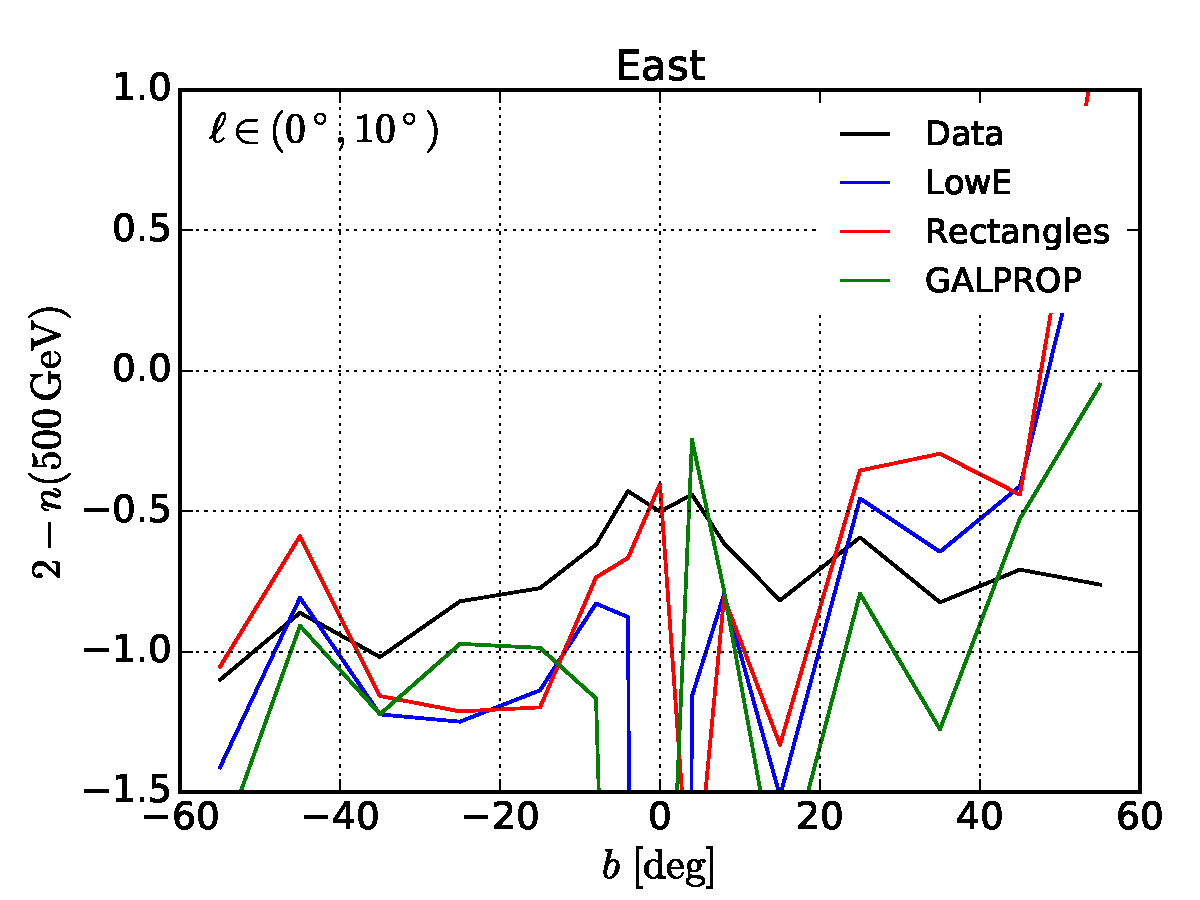
\includegraphics[width=0.5\textwidth]{plots/LogParabola_n(500GeV)_l_in_(0,10).pdf}
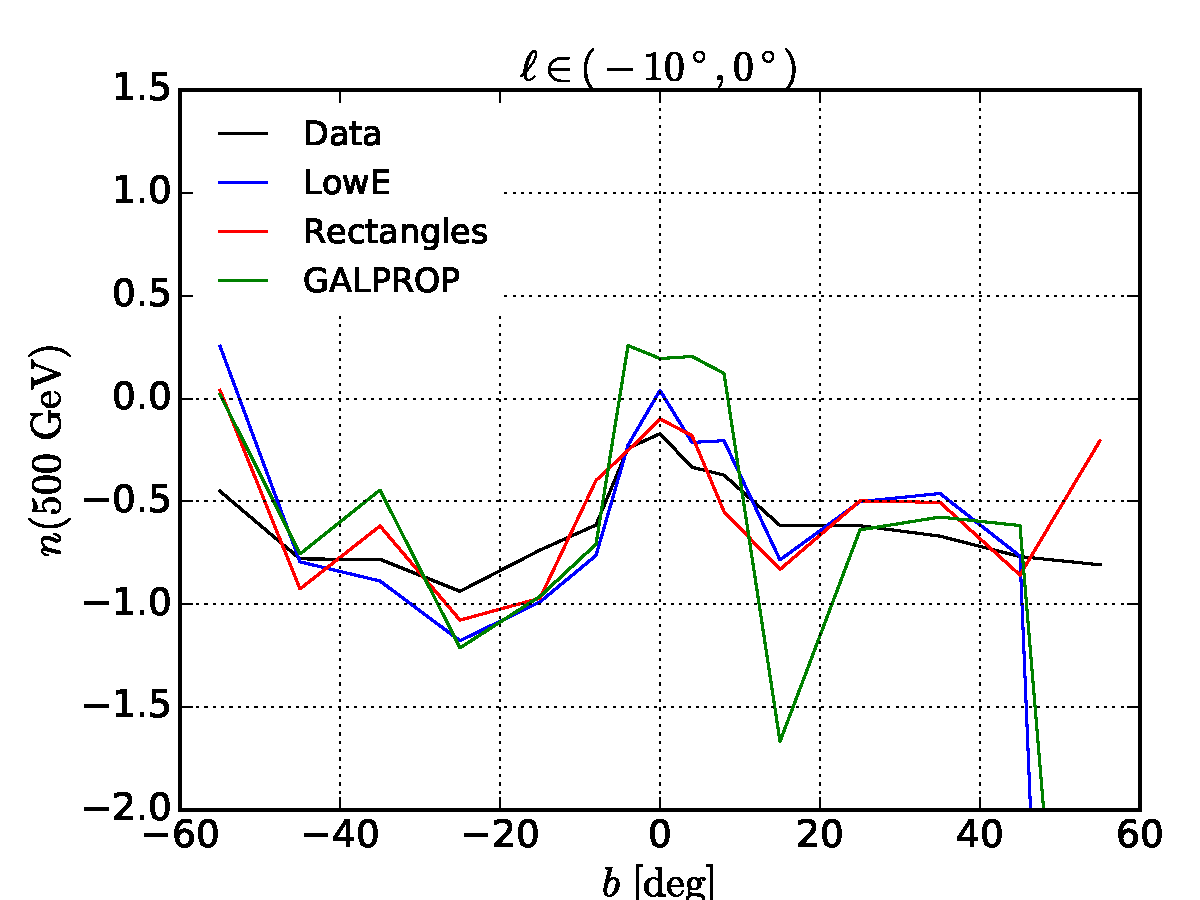
\includegraphics[width=0.5\textwidth]{plots/LogParabola_n(500GeV)_l_in_(-10,0).pdf}
\caption{
Index of the log-parabola defined in Equation (\ref{eq:log_par}) at  $E = \SI{500}{GeV}$ as a function of latitude for the FBs in 
the different foreground diffuse emission models.
%The width of the regions in longitude is $\ang{10}$, i.e. $\ang{0} - \ang{10}$ to the east of the GC (left) and $\ang{-10} - \ang{0}$ to the west of the GC (right).
}
\label{fig:logpar_index}
\end{figure*}


\subsection{Parametric model of the gamma-ray spectrum at low latitudes}
\label{sec:param_model}

In this section we study the spectrum of the FBs at latitudes $|b| < 6^\circ$.
As a baseline model we use the rectangles model of the FBs.
We compare a power-law model of the energy spectrum with a power-law and an exponential cutoff model
\be
\frac{dN}{dE} = N_0 \left( \frac{E}{1\:{\rm GeV}} \right)^{-n} e^{-E / E_{\rm cut}}.
\ee
The best-fit parameters for the rectangles model are reported in Table \ref{tab:param}.
If the improvement in $-2 \Delta \log \La$ is less than 0.1, then we report the power-law model parameters.
For the model with a cutoff, we also find the 95\% statistical confidence lower limit for the cutoff energy.
At last, we find the minimum among the 95\% confidence lower limits for all considered models.
The spectrum of the residuals including the FBs at  $\ell \in (\ang{-10},\ \ang{0})$
is consistent with a power law with an index $2.1 - 2.2$ up to $E \approx 1$ TeV.
The 95\% confidence lower limit on the cutoff energy is $\sim$ 300 GeV.
%\dima{Report the total luminosity (assuming the GC location) in erg/s including modeling ``error bars",  we can also do it in Section \ref{sec:GC_scenario}.}

\begin{table*}
  \begin{center}
    \caption{Parametric model of the FBs. We report the best fit values of the spectrum, the significance of the cutoff, 
    and statistical 95\% confidence lower limit on the cutoff for the rectangles model, $E_{\rm cut, 95\%}$.
    The last column is the minimal 95\% statistical lower limit among all models, $E_{\rm cut, 95\%}^{\rm min}$.
    There are four cases when the introduction of a cutoff does not lead to improved fit: in all of these cases
    $-2 \Delta \log \La < 0.1$ while the formal best-fit values of $E_{\rm cut}$ are larger than 1 TeV.
    The numbers in parenthesis in the last two columns show the results without the last energy bin.
    %\dima{Some numbers seem to be very different with and without the last data point, e.g., 2.4 (180) and 12 (130). I've marked the strange numbers in red. Also the 95\% cutoff values for the rectangles model without the last point seem to be higher in all cases, I'd expect that they would be almost always lower.}
    \Laura{I had normalized the powerlaw of the parametric model to 10 GeV. The correct values (for 1 GeV) are in parenthesis. IC and pi0 are not affected by the bug.}
    %\dima{I'm curious why the rectangles model is also the min model for negative longitudes in the Gal plane, for $\pi^0$ and IC models
    %the cutoffs are different in this region. I've marked what looked strange to me in red.}
    }
    \label{tab:param}
    \begin{tabular}{|c|c|c|c|c|c|c|c|} % <-- Alignments: 1st column left, 2nd middle and 3rd right, with vertical lines in between
     	\hline
		 Lat & Lon  & $N_0$ & $n$ & $E_{\rm cut}$ &  $-2 \Delta \log \La$ & $E_{\rm cut, 95\%}$ & $E_{\rm cut, 95\%}^{\rm min}$ \\ 
		       &        &  {\small $\SI{e-6}{GeV^{-1}cm^{-2}s^{-1} sr^{-1}}$ }&  & {\small $\SI{}{GeV}$ }& &{\small  $\SI{}{GeV}$ }&{\small  $\SI{}{GeV}$ }\\ 
		\hline
  		$(\ang{2}, \ang{6})$ & $(\ang{0}, \ang{10})$ & 1.9  \Laura{1.5}& 1.9 & 45 (45)& 4.8 & 25 (25) & 25  (25)\\ 
		& $(\ang{-10}, \ang{0})$ & 2.0 \Laura{3.1} & 2.2 & $-\ (690)$ \cmt{5.2e3} & $< 0.1$ \cmt{0.027} & {510 (210)} & {510} (210)  \\ 
 		\hline
  		$(\ang{-2}, \ang{2})$ & $(\ang{0}, \ang{10})$  & 3.5 \Laura{6.4}  & 2.3 & $-\ (610)$ \cmt{8.3e3} &  $< 0.1$ \cmt{0.010} & {300(180)}  & 2.4 (2.0)  \\ 
		& $(\ang{-10}, \ang{0})$  & 6.4 \Laura{7.9} & 2.1 & $-\ (1300)$ \cmt{8.3e6} &  $< 0.1$ \cmt{3.3e-5} & {{1000} (480)} & {1000}  (460)  \\ 
 		\hline
  		$(\ang{-6}, \ang{-2})$ & $(\ang{0}, \ang{10})$  & 1.8 \Laura{2.5} & 2.1 & 260 (260) & 3.8 & 130 (130)& {2.3 (2.3)} \\ 
		& $(\ang{-10}, \ang{0})$ & 2.8 \Laura{4.0} & 2.2 &  $-\ (780)$ \cmt{77e3} &  $< 0.1$ \cmt{0.020} & {560(290)}  & {560 (290)}  \\ 
 \hline
    \end{tabular}
  \end{center}
\end{table*}

\begin{table*}
  \begin{center}
    \caption{Rectangles model without last data point.}
        \begin{tabular}{|c|c|c|c|c|c|c|c|} % <-- Alignments: 1st column left, 2nd middle and 3rd right, with vertical lines in between
     	\hline
		 Lat & Lon  & $N_0$ & $n$ & $E_{\rm cut}$ &  $-2 \Delta \log \La$ & $E_{\rm cut, 95\%}$ & $E_{\rm cut, 95\%}^{\rm min}$ \\ 
		     &        &  {\small $\SI{e-6}{GeV^{-1}cm^{-2}s^{-1} sr^{-1}}$ }&  & {\small $\SI{}{GeV}$ }& &{\small  $\SI{}{GeV}$ }&{\small  $\SI{}{GeV}$ }\\ 
		\hline
  		$(\ang{2}, \ang{6})$ & $(\ang{0}, \ang{10})$ & 1.9 & 1.9 & 45 & 4.8 &25 & 25\\ 
		& $(\ang{-10}, \ang{0})$ & 2.0 & 2.2 & 690 & $< 0.1$ & 210 & 210\\ 
 		\hline
  		$(\ang{-2}, \ang{2})$ & $(\ang{0}, \ang{10})$ & 3.6 & 2.3  & 610 & $< 0.1$ & 180 & 2.0 \\ 
		& $(\ang{-10}, \ang{0})$ & 6.4 & 2.1 & 1.3e3 & $< 0.1$ & 480 & 460\\ 
 		\hline
  		$(\ang{-6}, \ang{-2})$ & $(\ang{0}, \ang{10})$ & 1.8 & 2.1 & 260 & 3.8 & 130 & 2.3  \\ 
		& $(\ang{-10}, \ang{0})$ & 2.9 & 2.1 & 780 & $< 0.1$ & 290 & 290\\ 
 \hline
    \end{tabular}
  \end{center}
\end{table*}


\subsection{IC model of the gamma-ray emission}
\label{sec:IC_model}

In this section we model the gamma-ray emission at the base of the FBs with an IC scattering model.
The SED of the gamma-ray intensity is

\be
E^2_\g \frac{dF_\g}{dE_\g} = 
\frac{E_\g c}{4\pi}\int \int \left(\frac{\de n}{\de E}\right)_{\!\!\ISRF} \sigma_\IC\ \left(\frac{\de \Sigma}{\de E}\right)_{\!\!\el} \de E_\ISRF\, \de E_\el,
\ee
where $\left(\frac{\de \Sigma}{\de E}\right)_{\!\!\el} = \int \left(\frac{\de n}{\de E}\right)_{\!\!\el} dR$ is the column density 
of CR electrons integrated along the line-of-sight radius $R$,
$(\de n/ \de E)_\ISRF$ is the number density of ISRF photons,
and $\sigma_\IC(E_\gamma, E_\ISRF, E_\el)$
is the differential IC scattering cross section in units of $E_\g\frac{d\sigma}{d E_\g}$ \citep{1970RvMP...42..237B}.
For details on the parametrization of $\sigma_\IC$ see Appendix B of \cite{2014ApJ...793...64A}.
The ISRF number density for starlight and IR photons is taken from GALPROP v54 \citep{2006ApJ...640L.155M}.
For the CMB, we use the thermal spectrum with a temperature of $\SI{2.73}{K}$.
We model the column density of electrons as a power law with a cutoff

\be 
\label{eq:e_spectrum}
\left(\frac{\de \Sigma}{\de E}\right)_{\!\!\el} = n_\el \left(\frac{E_\el}{\SI{1}{GeV}}\right)^{-\gamma_\el} e^{- E / E_{\cut}}.
\ee
In order to determine the normalization $n_\el$, the spectral index $\gamma_\el$, and the cutoff  $E_{\cut}$, 
we fit the IC model of the FBs plus the (fixed) foreground model counts to the 
total smoothed gamma-ray counts in different latitude stripes using likelihood based on gamma distribution.
As a baseline case, we take the gamma-ray spectrum derived in the rectangles model of the FBs in Section \ref{sec:box_model}.
The best-fit parameters for the rectangles model of the bubbles are reported in Figure \ref{fig:SED_with_fits}
%Figure \ref{fig:SED_with_fits} shows the residual of the rectangles model within 
in latitude stripes $b \in (\ang{2}, \ang{6})$, $b \in (-\ang{2}, \ang{2})$ and $b \in (-\ang{6}, -\ang{2})$. 
%The dotted line represents the best-fit IC spectrum for an electron distribution following a simple power law.
%\Laura{Should we here compare with the spectral indices of the other models?} \dima{yes}
%The spectral index to the west of the GC of the electron spectrum is harder than the spectrum to the east of the GC. 
If the improvement in $-2 \Delta \log \La$ with and without the cutoff is less than 0.1, then we show only the parameters for the power-law model without a cutoff.
For example, for negative longitudes the cutoff is not significant.

The 95\% statistical lower limit on the cutoff energy for the rectangles model and the minimum among all models of the 95\% confidence lower limits for the cutoff energy
are presented in Table \ref{tab:IC}.
%We also report the 95\% lower limit on the cutoff value. 
For negative longitudes,
the 95\% confidence lower limit on the cutoff in the spectrum of electrons in the rectangles model is about 4 TeV,
while the minimal value of the 95\% confidence limit for all the models of the foreground emission is about 3 TeV.


\begin{comment}
For that, we determine the photon counts detected by \Fermi-LAT that correspond to the IC radiation generated by the electrons in the respective region. For a volume $V$ and a distance $R$ to the region, the detected counts per energy bin $E$ are 
\be
N_{\gamma,\IC}(E) = \left(E\frac{\de n}{\de E}\right)_{\!\!\gamma,\IC} \cdot V \frac{\tau(E_\gamma)}{4 \pi R^2} \cdot \de(\log E_\gamma),
\ee
where $ \de(\log E_\gamma)$ is the logarithmic size of the energy bin. Since the exposure $\tau(E_\gamma)$, which is averaged over the area on the sky, depends on energy, it can affect the shape of the electron spectrum. The quantities $V$ and $R$ only affect the normalization of the electron spectrum and will not be important until section \ref{sec:Interpretation}.
The model for the total detected counts is the sum of one of the foreground models and the counts generated by the electron density via IC scattering. As our baseline model for the foreground, we pick the rectangles model.
 We fit our model of the total counts to the actually observed total counts in that region (with PS mask) using Poisson likelihood and extract the parameters $n_\el$ and $\gamma_\el$ of the electron spectrum.
\end{comment}


\begin{comment}
For $b \in (\ang{2}, \ang{6})$ the spectral index varies between 2.92 and 3.15 for the three models, for $b \in (-\ang{2}, \ang{2})$ between 2.68 and 3.54 and for $b \in (-\ang{6}, -\ang{2})$ between 2.85 and 3.00. The softest spectrum in each latitude stripe is fitted to the GALPROP model. To the east of the GC the spectral indices vary between 2.97 and 5.09 in the three latitude stripes. 

In order to test the presence of a cutoff in the spectrum of electrons, we fit the gamma-ray data using a spectrum of the electrons
with an additional cutoff factor $\exp(-\alpha E_\el)$, where $\alpha = E^{-1}_{\el,\cut}$ is the inverse cutoff.
The improvement in the $-2 \log \La$ \dima{We use Poisson log likelihood, right? I think it will be less confusing to use $-2 \log \La$,
which we actually calculate, rather  than $\chi^2$. We could even replace the two $\chi^2$ columns in the tables with a single column $-2 \Delta \log \La$,
since the actual values of $-2 \log \La$ do not mean much.}
for the models with and without the cutoff is shown in Table \ref{tab:IC}
for different latitude stripes.
\end{comment}



%We want to estimate the probability for the electron spectrum to have an exponential cutoff. For that we multiply an exponential cutoff $\exp(E_\el / E_{\el,\cut})$ to the electron spectrum \eqref{eq:e_spectrum} and determine the parameters analog to the procedure described before, using the rectangles model as the baseline foreground model.\\
%For the latitude stripe covering the Galactic plane, $b \in (-\ang{2}, \ang{2})$, adding a cutoff to the powerlaw does not improve the $\chi^2$-value both at negative ($\chi^2 \approx 135$) and positive longitudes ($\chi^2 \approx 128$).

%We determine the lower bound for the cutoff energy at a $\SI{95}{\percent}$-confidence level for our baseline model, the value in parenthesis gives the lowest value for all models: For negative longitudes we find a lower bound for the cutoff energy at $\SI{13.3}{TeV}$ ($\SI{2.9}{TeV}$), for positive longitudes at $\SI{491}{GeV}$ ($\SI{16}{GeV}$).

%Slightly below the Galactic plane, $b \in (-\ang{6}, -\ang{2})$, the $\chi^2$-value does not improve by exchanging the simple powerlaw by a powerlaw with a cutoff at negative longitudes ($\chi^2 \approx 76$). At positive longitudes the $\chi^2$-value improves slightly by adding the cutoff ($\chi^2 = 98$ to $\chi^2 = 87$). For negative longitudes we find a lower bound for the cutoff energy at $\SI{6.89}{TeV}$ ($\SI{6.89}{TeV}$), for positive longitudes at $\SI{818}{GeV}$ ($\SI{0.79}{GeV}$), at a $\SI{95}{\percent}$-confidence level.

\begin{figure*}[h!]
% version for the one-column style
%\begin{comment}
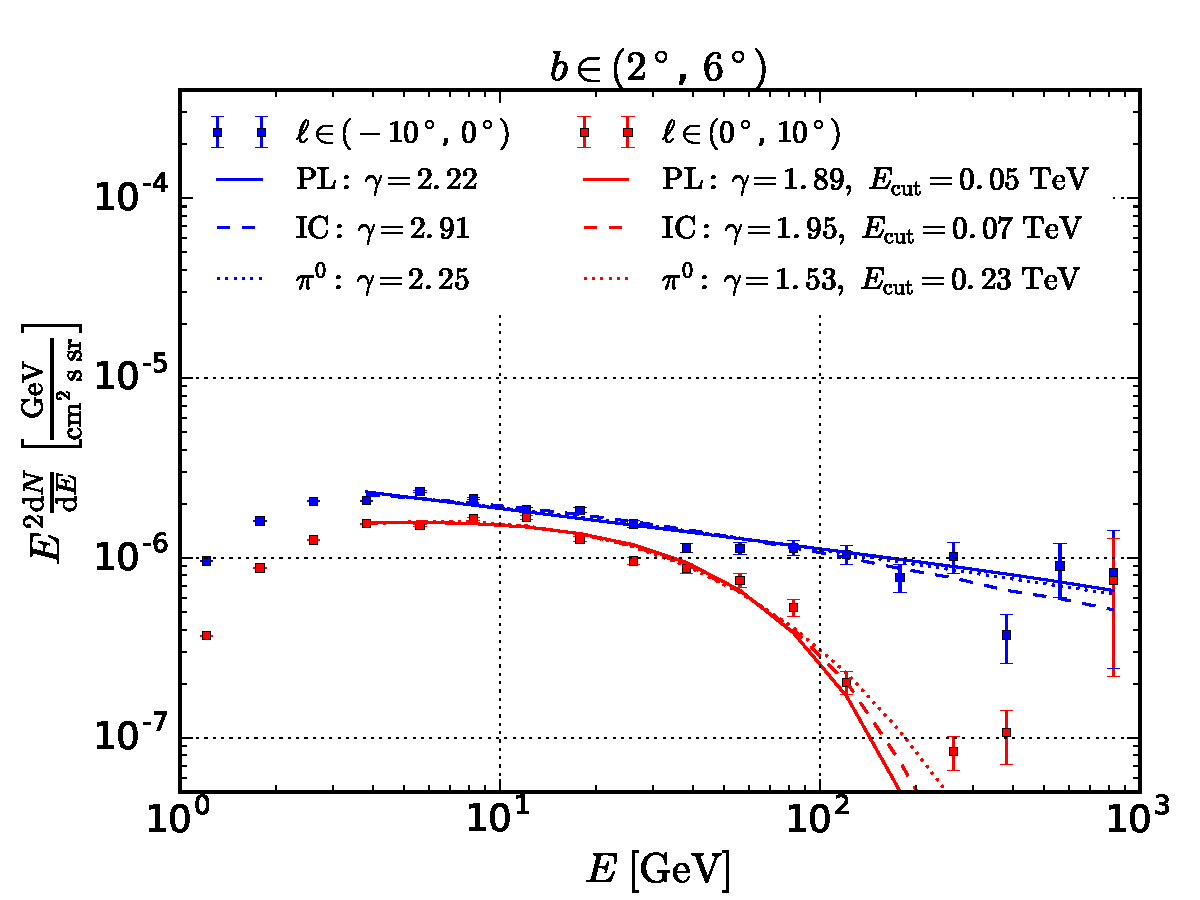
\includegraphics[width=0.33\textwidth]{plots/SED_boxes_source_4cutoff.pdf}
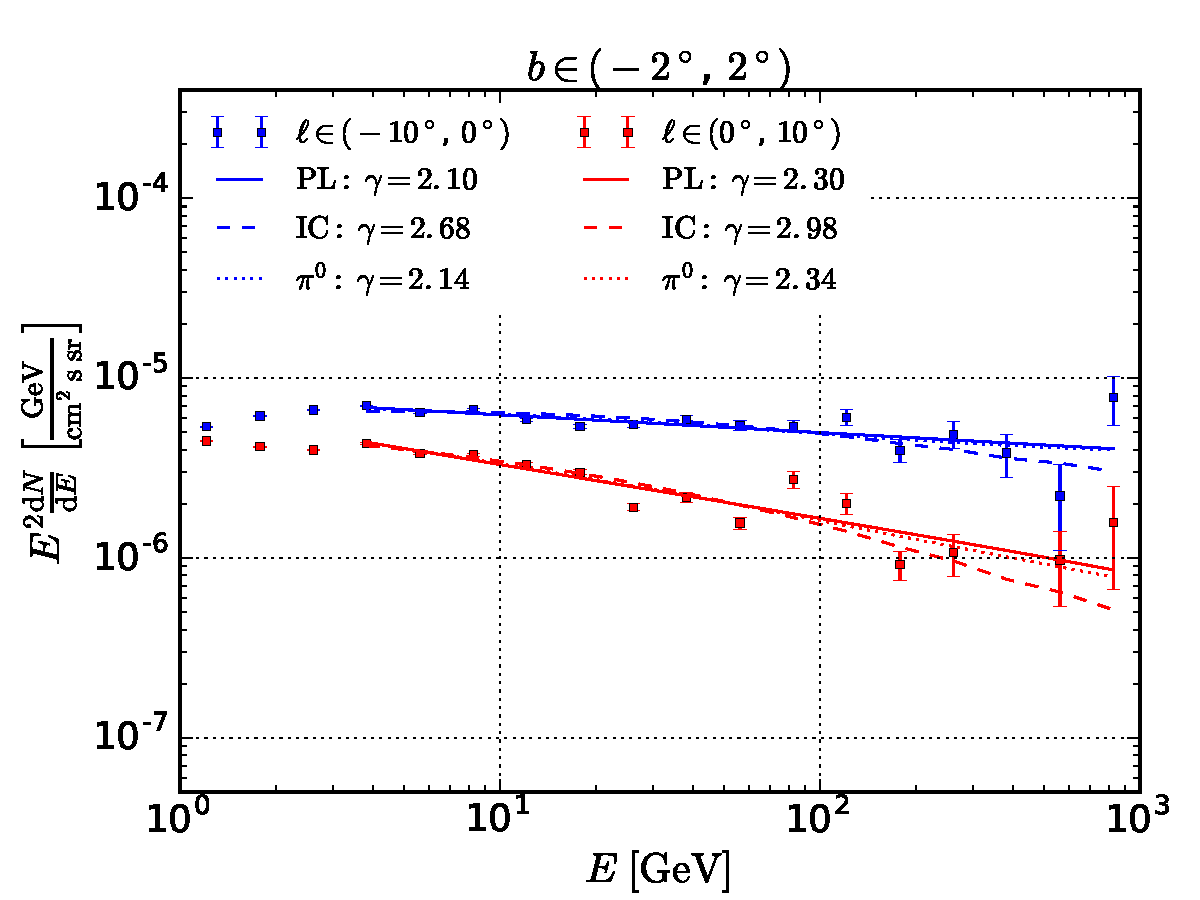
\includegraphics[width=0.33\textwidth]{plots/SED_boxes_source_0cutoff.pdf}
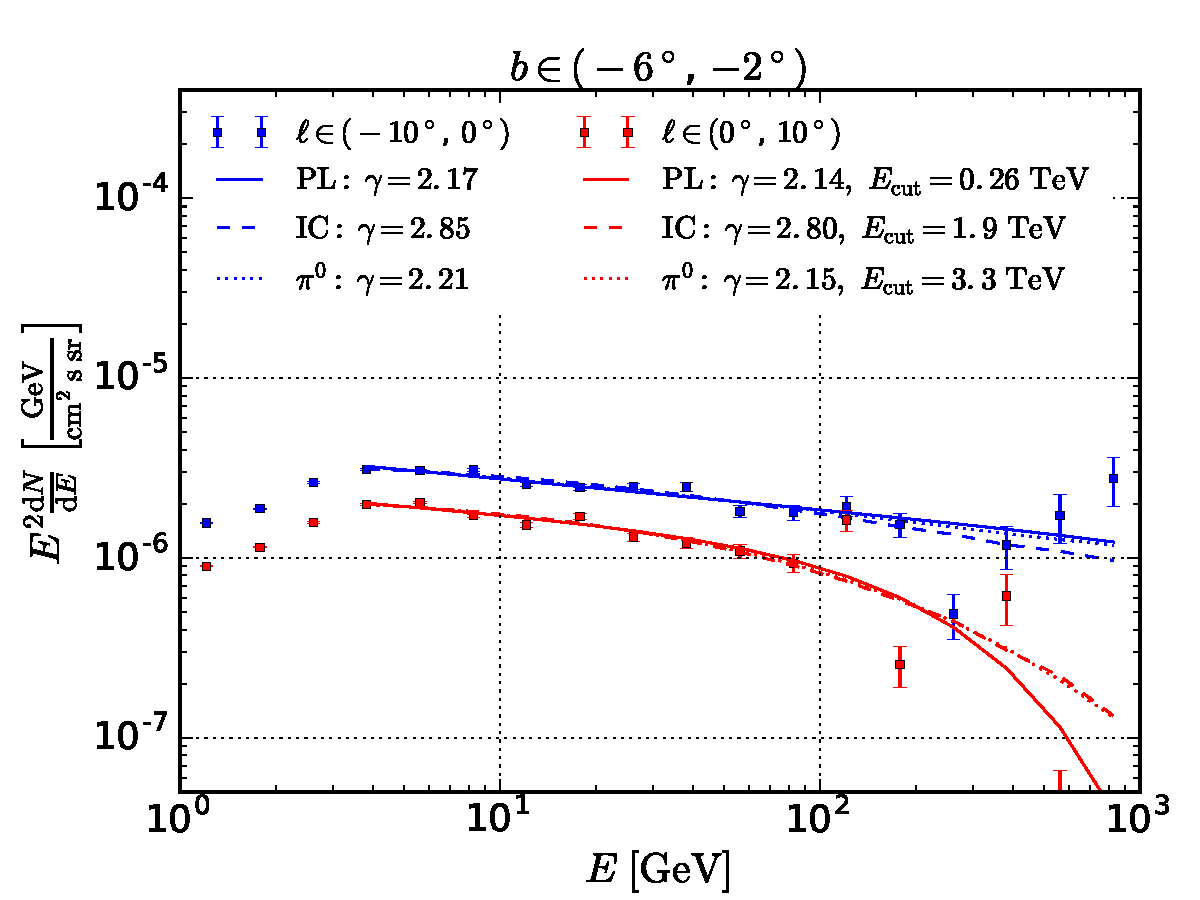
\includegraphics[width=0.33\textwidth]{plots/SED_boxes_source_-4cutoff.pdf}
%\end{comment}
% version for the two-column style?
\begin{comment}
    \begin{subfigure}{0.49\textwidth}
        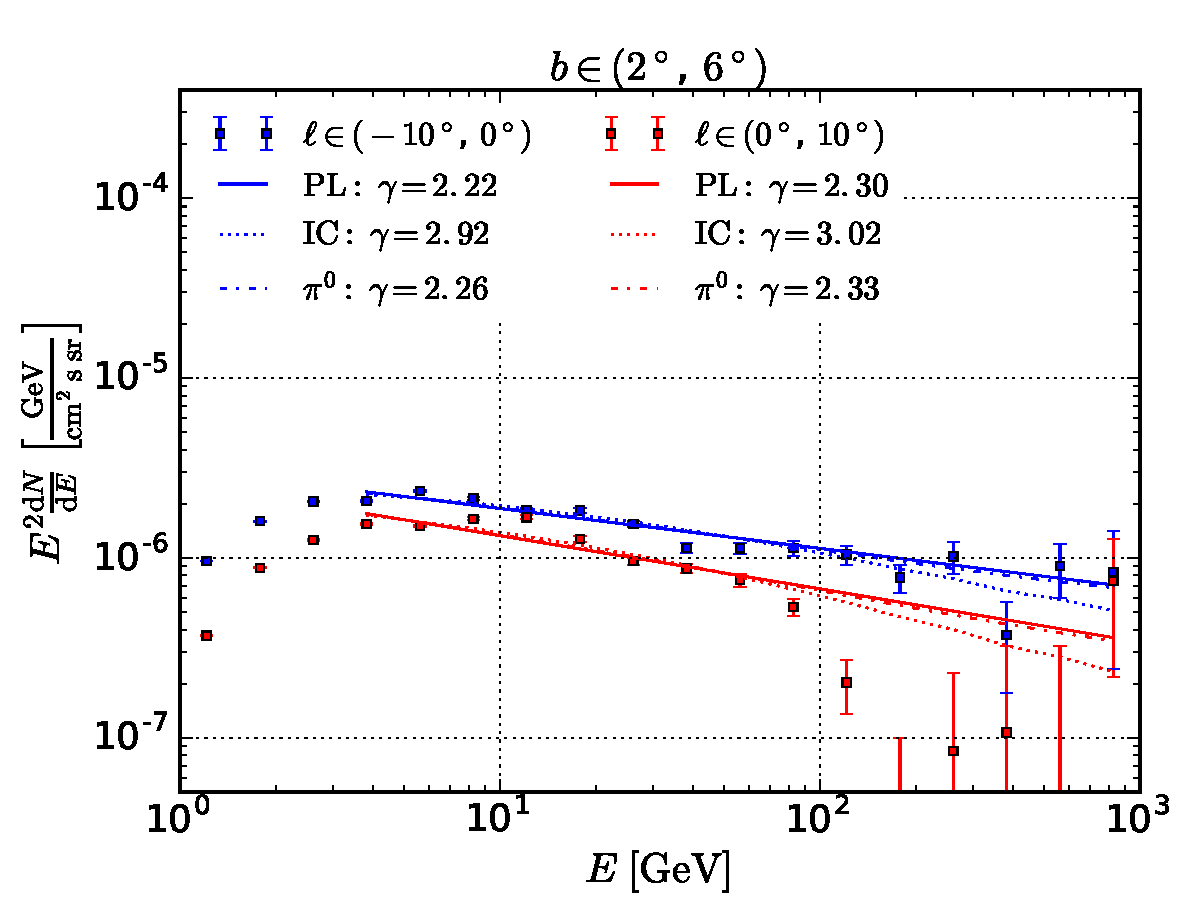
\includegraphics[width=\textwidth]{plots/SED_boxes_source_4.pdf}
    \end{subfigure}\\
    \begin{subfigure}{0.49\textwidth}
        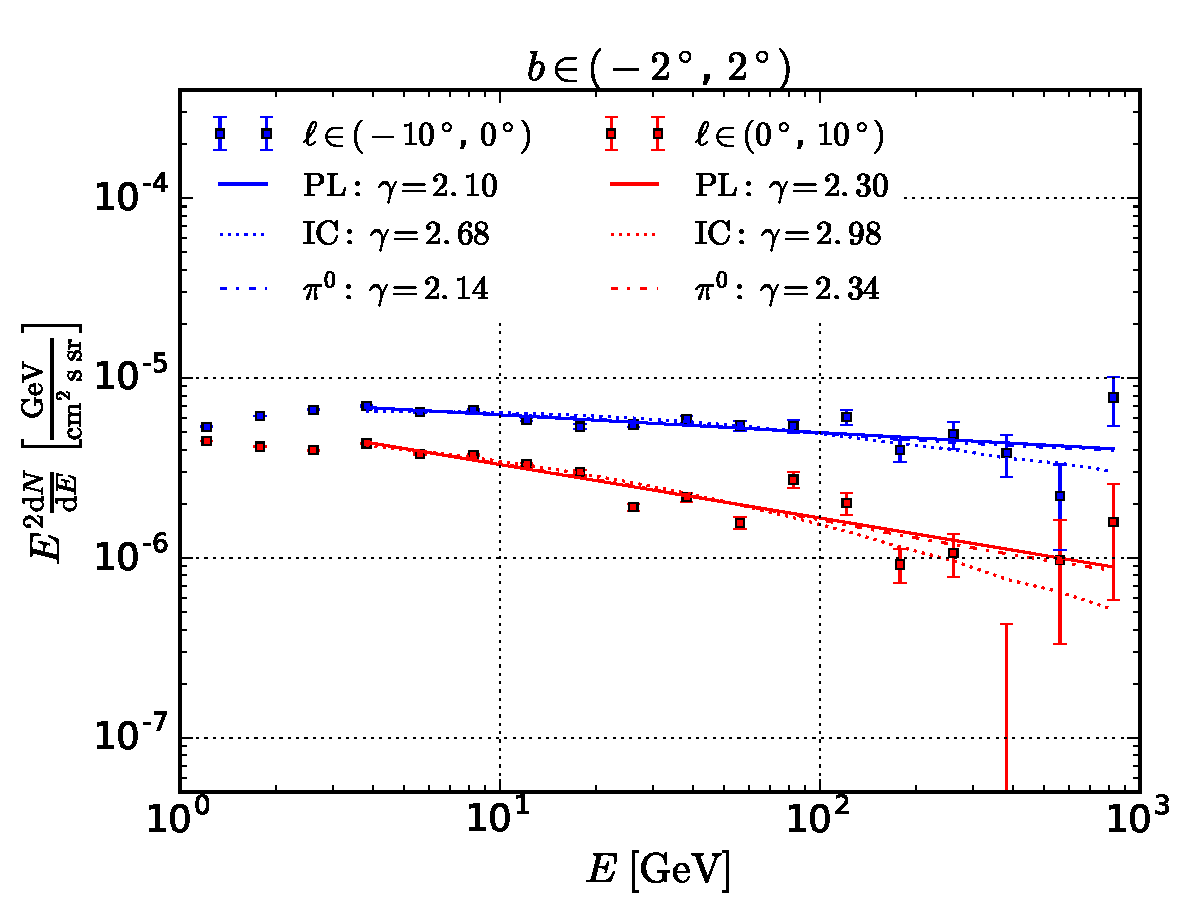
\includegraphics[width=\textwidth]{plots/SED_boxes_source_0.pdf}
    \end{subfigure} \\
    \begin{subfigure}{0.49\textwidth}
        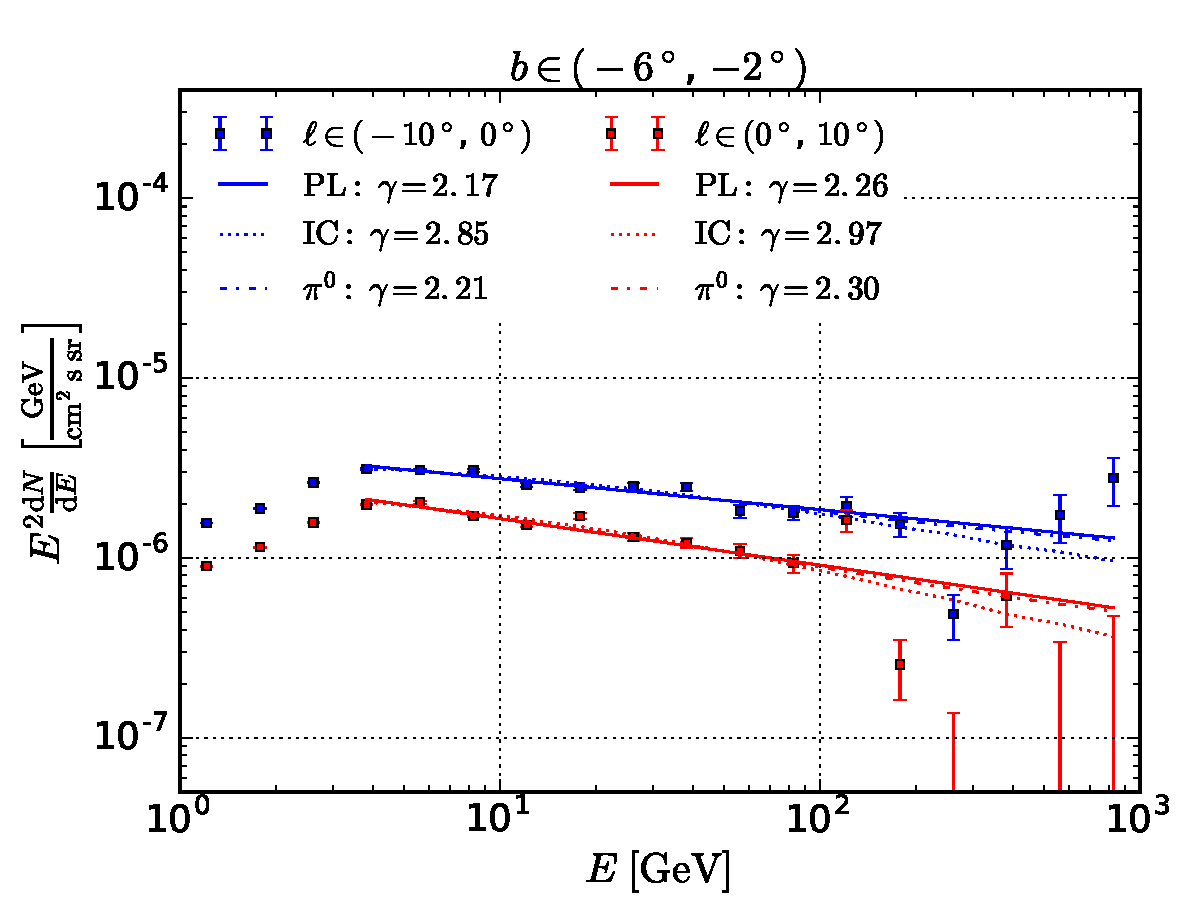
\includegraphics[width=\textwidth]{plots/SED_boxes_source_-4.pdf}
    \end{subfigure}
\end{comment}
  	\caption{SED of rectangles-model residual plus the FBs in the latitude stripes $(\ang{2}, \ang{6})$, $(\ang{-2}, \ang{2})$ and $(\ang{-6}, \ang{-2})$ for negative (blue) and positive (red) longitudes. We determine the spectral index of a power law (PL) of an electron distribution emitting gamma-rays via IC and of a proton distribution emitting gamma-rays via $\pi^0$-decay.}
  	%\Laura{Should we add the spectrum for the latitude band $(\ang{2}, \ang{6})$ also, or just say that it looks similar?}
	%\blue{Dima: yes, let's add the 2 to 6 deg spectrum.}
  	\label{fig:SED_with_fits}
\end{figure*}

%
%\begin{center}
%\begin{tabular}{ |c|c|c|c|c| } 
% \hline
% lat & lon  & $\chi^2$(no cutoff) &  $\chi^2$(cutoff) & Lower bound $E_\cut$ \\ 
% \hline
%  2 -- 6 & east & $\chi^2$(no cutoff) &  $\chi^2$(cutoff) & Lower bound $E_\cut$\\ 
%2 -- 6 & west & $\chi^2$(no cutoff) &  $\chi^2$(cutoff) & Lower bound $E_\cut$ \\ 
% \hline
%   -2 -- 2 & east & $\chi^2$(no cutoff) &  $\chi^2$(cutoff) & Lower bound $E_\cut$\\ 
%-2 -- 2 & west & $\chi^2$(no cutoff) &  $\chi^2$(cutoff) & Lower bound $E_\cut$\\ 
% \hline
%  -6 -- -2 & east & $\chi^2$(no cutoff) &  $\chi^2$(cutoff) & Lower bound $E_\cut$\\ 
%-6 -- -2 & west & $\chi^2$(no cutoff) &  $\chi^2$(cutoff) & Lower bound $E_\cut$\\ 
% \hline
%\end{tabular}
%\end{center}

\begin{table*}
  \begin{center}
    \caption{Energy cutoff values and the significance of the cutoff in the IC model of the FBs at low latitudes.
%  $\chi^2$-values for IC-spectrum fit of a distribution of electrons following a simple powerlaw and a powerlaw with cutoff, respectively in the latitude bands discussed in the text. 
The lower bounds for $E_\cut$ at the 95\% confidence level for our baseline model and the minimum among all
models are shown in the last two columns respectively.
}
    \label{tab:IC}
    \begin{tabular}{|c|c|c|c|c|} % <-- Alignments: 1st column left, 2nd middle and 3rd right, with vertical lines in between
     	\hline
		 Lat & Lon  & $-2 \Delta \log \La$ & \multicolumn{2}{c|}{Lower bound on $E_\cut$ (TeV) } \\ 
		       &        &                                  &  \multicolumn{1}{c}{Rectangles model} & All models \\ 
		\hline
  		$(\ang{2}, \ang{6})$ & $(\ang{0}, \ang{10})$ & 2.6  & 0.05 \Laura{0.20} & 0.05 \Laura{0.17}\\ 
		& $(\ang{-10}, \ang{0})$ & $ < 0.1$  & 4.0  & 4.0 \\ 
 		\hline
  		$(\ang{-2}, \ang{2})$ & $(\ang{0}, \ang{10})$ & $ < 0.1$ & 1.5 \Laura{1.4} & 0.01 \\ 
		& $(\ang{-10}, \ang{0})$ & $ < 0.1$ & 13  & 2.9  \\ 
 		\hline
  		$(\ang{-6}, \ang{-2})$ & $(\ang{0}, \ang{10})$ & 1.1 & 0.83 \Laura{0.82} & 0.03 \\ 
		& $(\ang{-10}, \ang{0})$& $ < 0.1$ & 6.3 \Laura{7.0} & 6.3 \Laura{7.0} \\ 
 \hline
    \end{tabular}
  \end{center}
\end{table*}




%\begin{figure}
%	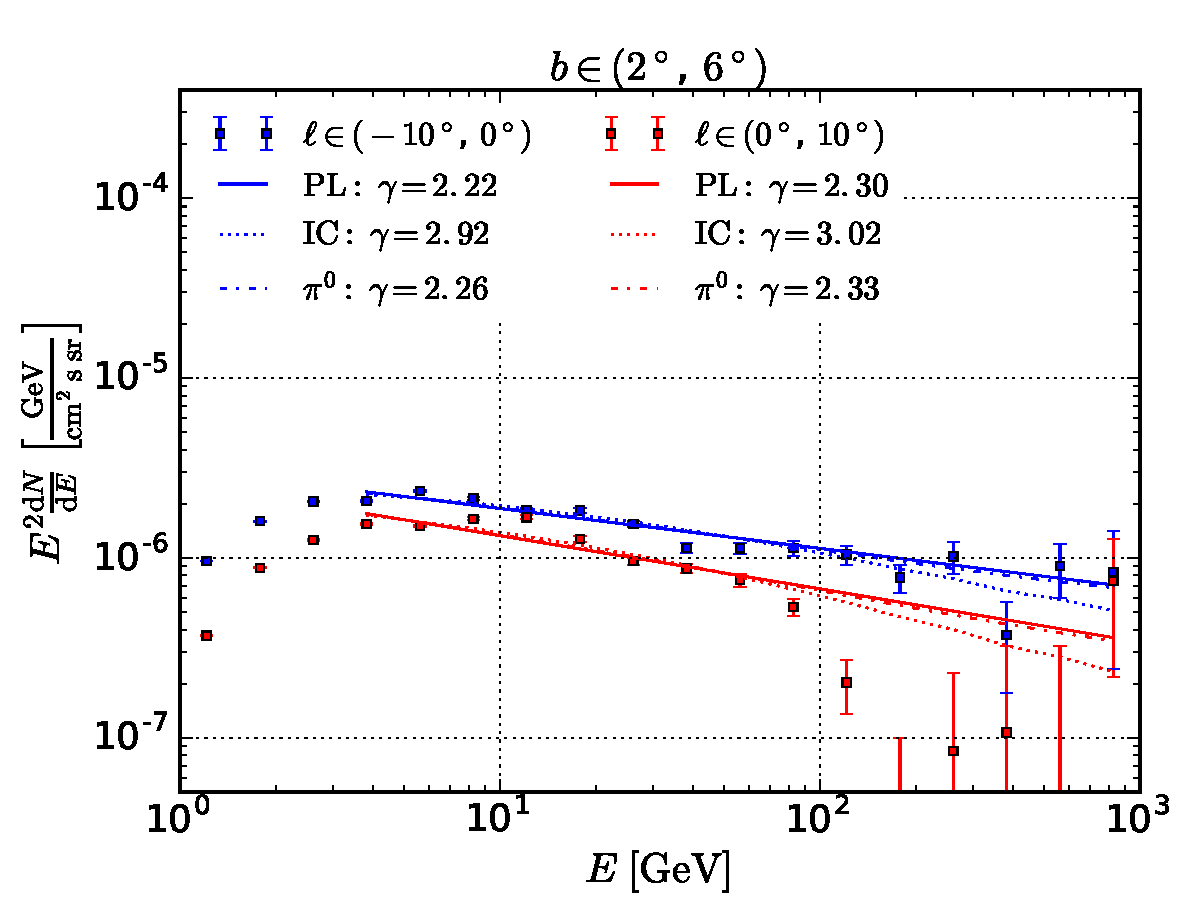
\includegraphics[width=0.5\textwidth]{plots/SED_boxes_source_4.pdf}
%\end{figure}
%\begin{figure}
%	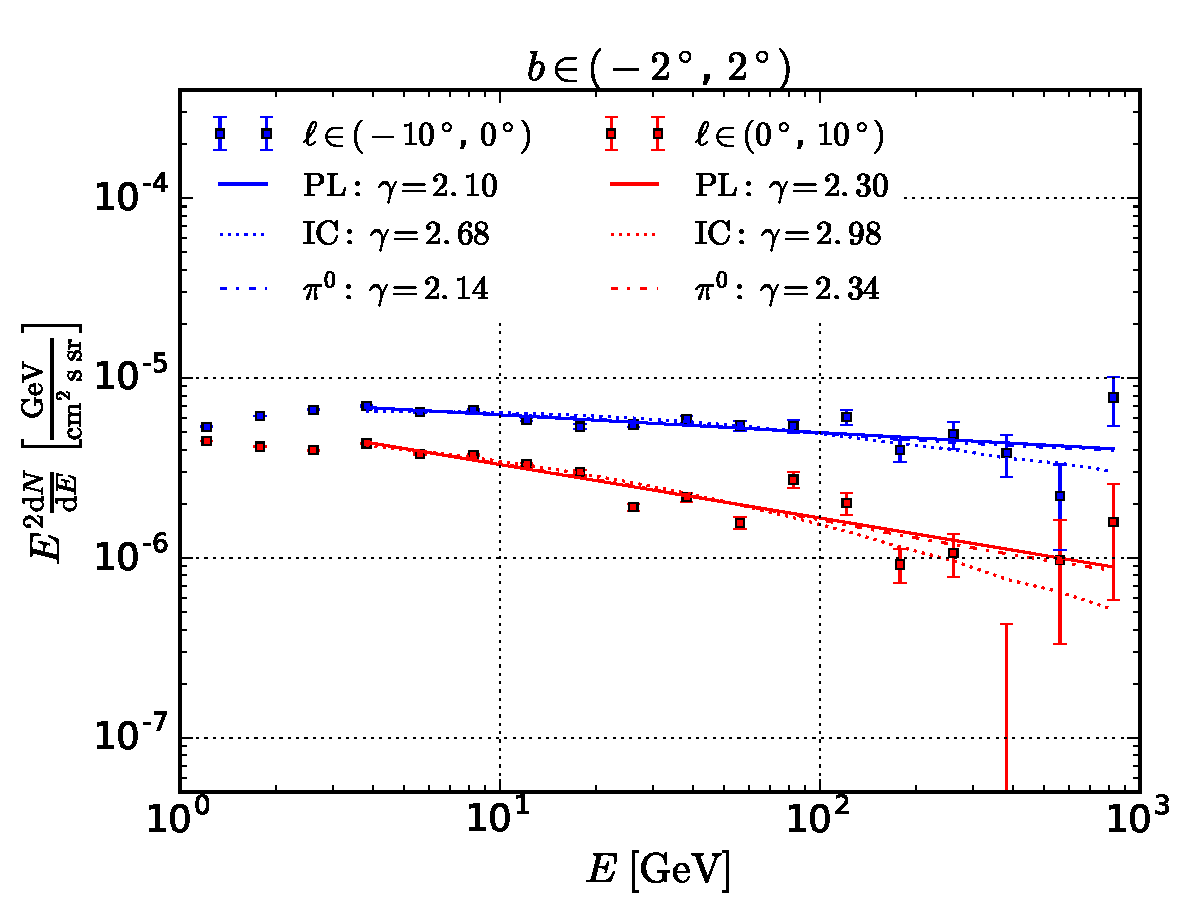
\includegraphics[width=0.5 \textwidth]{plots/SED_boxes_source_0.pdf}
%\end{figure}
%\begin{figure}
%	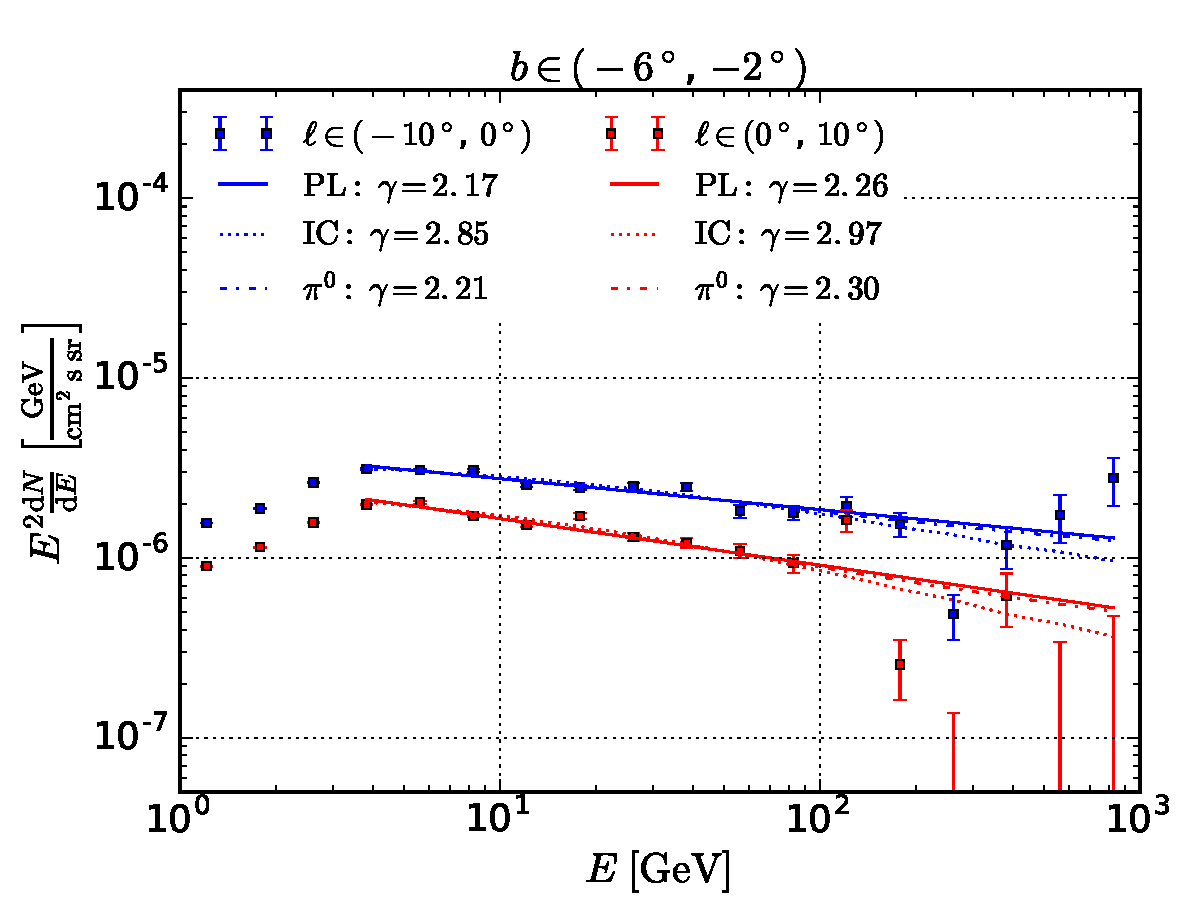
\includegraphics[width=0.5\textwidth]{plots/SED_boxes_source_-4.pdf}
%	\caption{SED of rectangles-model residual in the latitude stripes $(\ang{-2}, \ang{2})$ (left) and $(\ang{-6}, \ang{-2})$ (right) for negative (blue) and positive longitudes (red). We determine the spectral index of a powerlaw (PL), of an electron distribution emitting gamma-rays via IC and of a proton distribution emitting gamma-rays via $\pi^0$-decay.}
%\end{figure}


\subsection{Hadronic model of gamma-ray emission}
\label{sec:Pion_model}

In the hadronic model, the gamma rays are produced as a result of collisions of hadronic CR with the interstellar gas.
The gamma-ray intensity in the hadronic model is

\be
E^2_\g \frac{dF_\g}{dE_\g} = \frac{E_\g}{4\pi} \int n_\Hy\ \sigma_\pr v_\pr \left(\frac{\de \Sigma}{\de T}\right)_{\!\!\pr} \de T_\pr,
%\frac{Ec}{4\pi}\int \int \left(\frac{\de n}{\de E}\right)_{\!\!\ISRF} \sigma_\IC\ \left(\frac{\de \Sigma}{\de E}\right)_{\!\!\el} \de E_\ISRF\, \de E_\el,
\ee
where $\left(\frac{\de \Sigma}{\de E}\right)_{\!\!\pr} = \int \left(\frac{\de n}{\de E}\right)_{\!\!\pr} dR$ is the column density 
of CR protons,
$T_\pr = \sqrt{(q c)^2 + (m_p c^2)^2} - m_p c^2$ is the kinetic energies of the protons,
$n_\Hy$ is the density of gas, and $\sigma_\pr (E_\gamma, T_\pr)$ is 
the differential cross section in units of $E_\g\frac{d\sigma}{d E_\g}$
for gamma rays in proton-proton collisions \citep{2006ApJ...647..692K, 2008ApJ...674..278K}.
We model the proton spectrum as a power law of the momentum $\frac{d \Sigma}{d qc} = n_\pr q^{-\g_p}$ 
(note, that $ v \frac{\de \Sigma}{\de T} = c \frac{d \Sigma}{d qc}$).

We fit the hadronic model of the gamma-ray emission at the base of the FBs analogously to the leptonic model in 
Section \ref{sec:IC_model}.
%We add the hadronic model of the gamma-ray emission at the base of the FBs to the foreground emission 
%and determine the normalization $n_\pr$ and index $\gamma_\pr$ of the CRp spectrum
%by fitting the total model to the \Fermi-LAT data using Poisson log likelihood.
The dash-dotted line in Figure \ref{fig:SED_with_fits} represents the best-fit hadronic spectrum (labeled as $\pi^0$). 
The index of the proton spectrum is relatively hard $\g_\pr \lesssim 2.3$, especially to the west of the GC.
\begin{comment}
For that, we again fit the sum of the photon counts generated by hadronic processes and the baseline model for the foreground to the total photon counts detected by the \Fermi-LAT (with PS mask) using Poisson likelihood.  
For $b \in (\ang{2}, \ang{6})$ the spectral index to the west of the GC varies between 2.26 and 2.42, for $b \in (-\ang{2}, \ang{2})$ between 2.14 and 2.64 and for $(-\ang{6}, -\ang{2})$ between 2.21 and 2.32. To the east of the GC the indices vary between 2.33 and 3.55. 
\end{comment}

We calculate the significance of a cutoff in the CR proton spectrum by adding an exponential cutoff factor and refitting the model to the gamma-ray data.
The improvement in the model and the 95\% confidence lower bound on the cutoff values are presented in Table \ref{tab:pi0}.
Within $\pm 6^\circ$ from the Galactic plane west of the GC, the 95\% confidence level for the lower bound on the cutoff among all the models
of the foreground emission that we have considered is about 1.6 TeV.


\begin{comment}
We again estimate the probability for the proton spectrum to have an exponential cutoff: For the latitude stripe covering the Galactic plane, $b \in (-\ang{2}, \ang{2})$, adding a cutoff does neither improve the $\chi^2$-valueat negative ($\chi^2 \approx 62$) nor positive longitudes ($\chi^2 \approx 116$). At a $95\%$-confidence level, the lower bound for the cutoff energy for the baseline model (and all models) is $\SI{28.6}{TeV}$ ($\SI{22.6}{TeV}$) for negative longitudes and $\SI{1.8}{TeV}$ ($\SI{11.5}{GeV}$) for positive longitudes.\\
In the latitude band $(-\ang{6}, -\ang{2})$, the $\chi^2$-value does increase both for negative ($\chi^2 = 157$ to $\chi^2 = 123$) and positive longitudes ($\chi^2 = 245$ to $\chi^2 = 156$) by adding an exponential cutoff. The lower bound on the cutoff energy is $\SI{23.6}{TeV}$ ($\SI{0.99}{TeV}$) for negative and $\SI{1.57}{TeV}$ ($\SI{40}{GeV}$) for positive longitudes.
\end{comment}


\begin{table*}
  \begin{center}
    \caption{\label{tab:pi0} 
Energy cutoff values and the significance of the cutoff in the hadronic model of the FBs at low latitudes.
%    $\chi^2$-values for hadronic-spectrum fit of a distribution of protons following a simple powerlaw and a powerlaw with a cutoff, respectively in the latitude bands discussed in the text. 
The lower bounds for $E_\cut$ at the 95\% confidence level for our baseline model and the minimum among all
models are shown in the last two columns respectively. 
}
    \begin{tabular}{|c|c|c|c|c|} % <-- Alignments: 1st column left, 2nd middle and 3rd right, with vertical lines in between
     	\hline
		 lat & lon  & $-2 \Delta \log \La$ & \multicolumn{2}{c|}{Lower bound on $E_\cut$ (TeV) } \\
		      &        &                                  &       \multicolumn{1}{c}{Rectangles model} & All models \\ 
		\hline
  		$(\ang{2}, \ang{6})$ & $(\ang{0}, \ang{10})$ & 4.4 & 0.16 \Laura{0.88} & 0.16 \Laura{0.48} \\ 
		& $(\ang{-10}, \ang{0})$ &  $ < 0.1$ & 1.6 \Laura{7.4} & 1.6 \Laura{7.4}\\ 
 		\hline
  		$(\ang{-2}, \ang{2})$ & $(\ang{0}, \ang{10})$ & $ < 0.1$ & 1.3 \Laura{3.8} & 0.023 \\ 
		& $(\ang{-10}, \ang{0})$ & $ < 0.1$ & 30 \Laura{29} & 6.3 \\ 
 		\hline
  		$(\ang{-6}, \ang{-2})$ & $(\ang{0}, \ang{10})$ & 2.7 & 1.6 & 0.05 \\ 
		& $(\ang{-10}, \ang{0})$ & $ < 0.1$ & 2.1 \Laura{12} & 2.1 \Laura{12}\\ 
 \hline
    \end{tabular}
  \end{center}
\end{table*}

\subsection{Summary of the spectral analysis}

In Figure \ref{fig:spec_summary} we show the envelopes of the gamma-ray spectra at $|b| < 2^\circ$ of the residuals plus FB
for the models of foreground emission that we have considered including the models where we change the selection of the low energies 
in the definition of the foreground emission model (Appendix \ref{sec:lowE_syst}).
In order to determine the maximal and minimal models of the FBs in the Galactic plane, 
we fit the maximal and minimal points in the envelope above 3 GeV with a power-law with a cutoff function
(we fit above 3 GeV because some of the models of the foreground emission in Appendix \ref{sec:lowE_syst} are determined 
for energies between 1 and 3 GeV).
The corresponding parameters are reported in the first raw of Table \ref{tab:summary}.
We also fit the IC and hadronic models to the maximal and minimal points in the envelope and report the corresponding parameters
in Table \ref{tab:summary}.


%\dima{we can put a summary plot with the baseline model and the band of all spectra in a small subsection here}

\begin{figure}[h]
\centering
 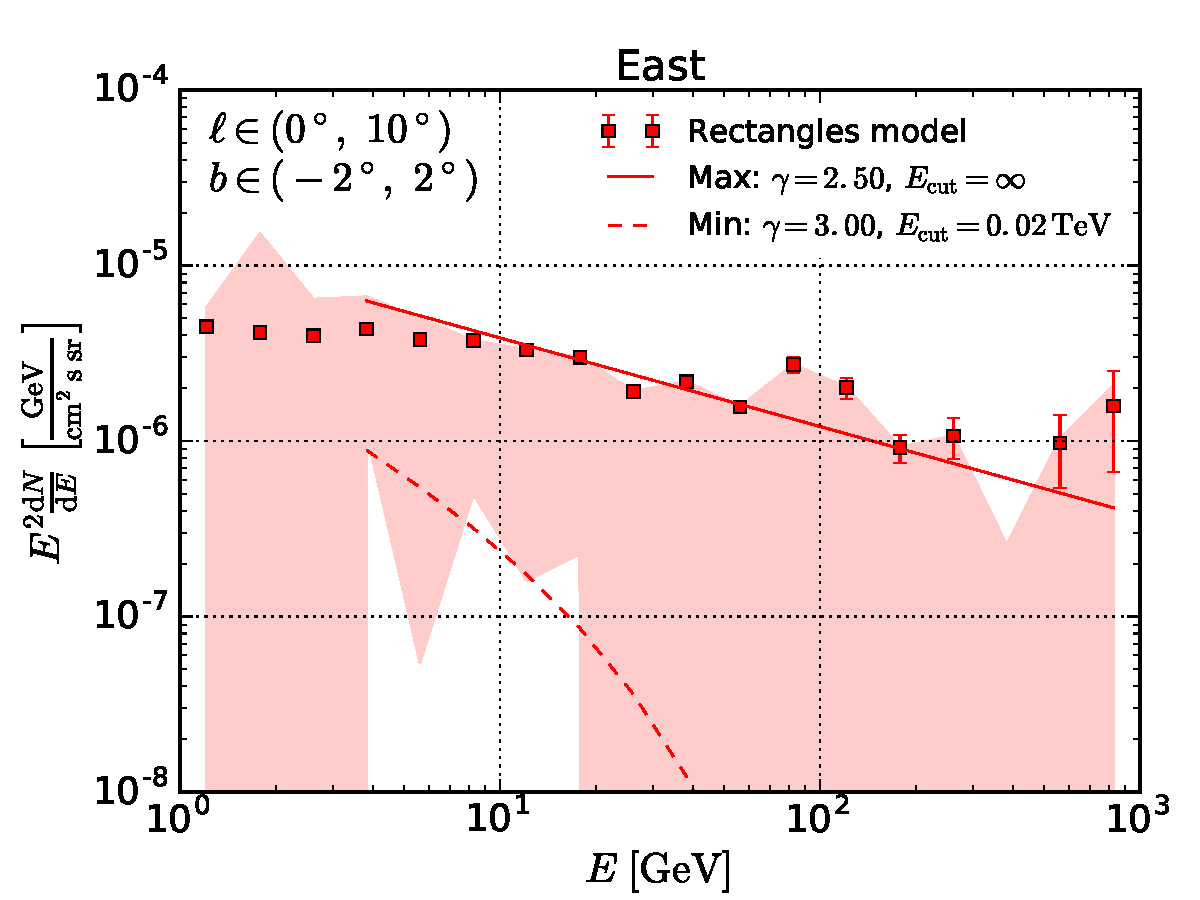
\includegraphics[width=0.48\textwidth]{plots/Summary_SED_b=0_l=5.pdf}
  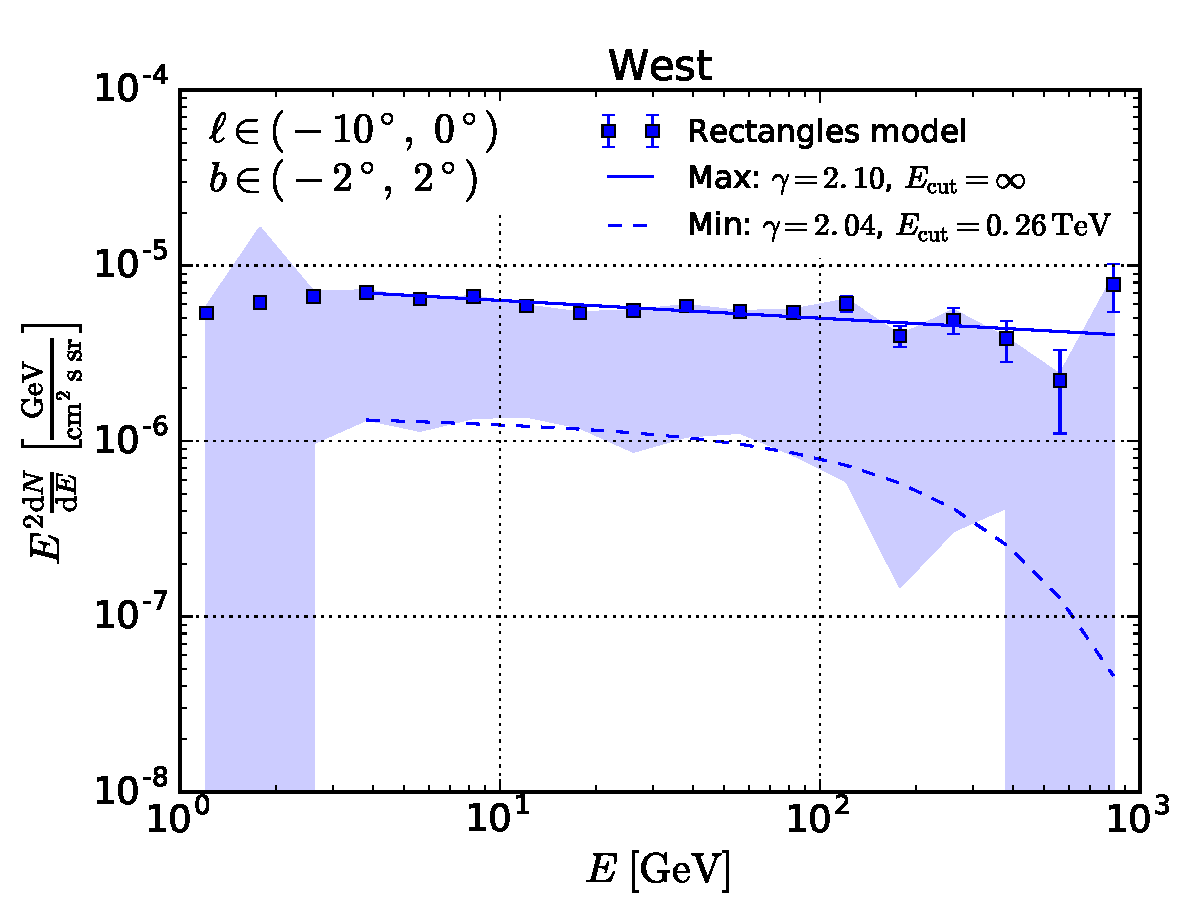
\includegraphics[width=0.48\textwidth]{plots/Summary_SED_b=0_l=-5.pdf}
 \caption{SED of the FBs in the Galactic plane. 
 The shaded areas show the envelope of the FBs spectra in all foreground models considered in the paper
including the changes in the choice of the low-energy range to model the foreground emission
(discussed in Appendix \ref{sec:lowE_syst}).
The lines show the fits to the maximal and minimal points in the envelopes above 3 GeV.
}
 \label{fig:spec_summary}
\end{figure}


\begin{table*}
  \begin{center}
    \caption{Summary of the min and max models for the parametric, 
    IC and hadronic models of the FBs for $|b| < 2^\circ$ and $-10^\circ < \ell < 0^\circ$. 
    For the parametric model, we report the energy spectrum of the gamma rays,
    for the IC model we report the surface density of the electrons spectrum as a function of energy,
    while for the hadronic model -- the surface density of the protons spectrum as a function of momentum.
    The spectra are normalized at $E_0 = 1$ GeV. The last column shows the statistical 95\% confidence lower limit on the cutoff, $E_{\rm cut, 95\%}$.}
    \label{tab:summary}
    \begin{tabular}{| l |c|c|c|c|c|c|c|} % <-- Alignments: 1st column left, 2nd middle and 3rd right, with vertical lines in between
     	\hline
		 {\hspace{2cm}Model} & Type  & norm & index & cutoff & $E_{\rm cut, 95\%}$ \\ 
		       &        &   &  & {\rm\small TeV} & {\rm\small TeV}\\ 
		\hline
  		\multirow{2}{*}{Parametric, $\frac{dN_\g}{dE}$ {\small $\left[{\rm {GeV^{-1}\, cm^{-2}\, s^{-1} }}\right]$}} & max & $\SI{8.0e-6}{} $ \red{8.1e-6} & 2.10 \red{2.11} &  -- & 3.9 \red{1.65} \\ 
		& min & $\SI{1.4e-6}{}$ \red{1.12e-6} & 2.04 \red{1.91} &  0.26 \red{0.11} & 0.14 \red{0.039} \\ 
 		\hline
  		\multirow{2}{*}{IC, $\frac{d\Sigma_e}{dE}$ {\small $\left[{\rm {GeV^{-1}\, cm^{-2}}}\right]$}} & max & $\SI{4.0e10}{}$ \red{33.5e9} & 2.71 \red{2.67} &  -- & 59 \red{18.5} \\ 
		& min & $\SI{5.6e9}{}$ \red{12.5e9} & 2.60 \red{2.81} &  1.1 \red{7.18} & 0.43 \red{0.96} \\ 
 		\hline
  		\multirow{2}{*}{Hadronic, $\frac{d\Sigma_p}{dqc}$ {\small $\left[{\rm {GeV^{-1}\, cm^{-2}}}\right]$}} & max & $\SI{1.0e12}{}$ \red{9.51e11} & 2.15\red{2.13} &  -- & 276 \red{64.9} \\ 
		& min & $\SI{1.1e11}{}$ \red{1.05e11} & 2.00 \red{1.98} &  2.3 \red{1.79} & 1.1 \red{0.23}  \\ 
 \hline
    \end{tabular}
  \end{center}
\end{table*}




\section{Conclusions}

For the ROI, $b \in (\ang{-2},\ang{2}),\ \ell \in (\ang{-10},\ang{0})$, the total energy density in electrons with energy above $E_0 = \SI{1}{GeV}$ is given by the integral of the electron spectrum that was found in Section \ref{sec:IC_model}:

\be
\frac{\de E_\tot}{\de V} = \int_{E_0}^{\infty} \left(E \frac{\de N}{\de E}\right)_\el \de E = \SI{3.8e-14}{erg/cm^3}.
\ee
Assuming a distance of $\SI{8}{kpc}$ to the ROI, the volume of the ROI is $V = \SI{0.54}{kpc^3} = \SI{1.58e64}{cm^3}$. The total energy content of the ROI in electrons above $\SI{1}{GeV}$ is $E_\tot = \SI{6e50}{erg}$, which corresponds to the CR energy output of $60$ SNe.\\
Using the result from Section \ref{sec:Pion_model} we find an energy density in protons of $\de E_\tot / \de V = \SI{6.6e-13}{erg/cm^3}$ and a total energy content of $E_\tot = \SI{1e52}{erg}$. However, the gas density in the inner Galaxy is probably higher than $n_\Hy = \SI{1}{/cm^3}$ as assumed in Section \ref{sec:Pion_model}, resulting in an energy content in protons of the same order of magnitude as the energy density in electrons. \\
\\
To estimate the maximal propagation distance of electrons, we start with a diffusion equation taking into account diffusion and energy loss $b_\IC(E)$ via IC. From the solution we read off the diffusion distance for electrons with energy $E_0 = \SI{1}{TeV}$:
\be
\langle x \rangle^2 = 2 \int_{E_0}^E \frac{D(E)}{b_\IC(E)}\de E = \SI{1300}{pc}.
\ee
with a spatially constant diffusion coefficient $D(E) = D_0\left(\frac{E}{\SI{1}{GeV}}\right)^\delta$, where we take values of the local diffusion coefficient: $D_0 = \SI{3e28}{cm^2/s} = \SI{100}{pc^2/kyr}$ and $\delta = 0.4$. The energy loss $b_\IC(E)$ is \dots. Since the diffusion distance of the electrons exceeds the spatial size of the ROI, the electrons cannot be confined. Therefore, we find that a transient process is favoured. The energy losses of protons exceed the energy losses of electrons by far, therefore the same applies for protons.\\
Wit the local diffusion coefficient we find an escape time for both electrons and protons of 
\be
T = \frac{\Delta x^2}{2 D(E)} = \SI{70}{kyr}.
\ee



\newpage
\bibliography{gp_bubbles_papers}  

\begin{appendix}
\section{Modeling uncertainties}

Include the models with different selection of low energies.
\newpage
\section{Gamma distribution as a likelihood for smoothed data}
\lb{app:gamma}

In this appendix we show that smoothing the data and using gamma distribution instead of the Poisson distribution
is a reasonable procedure (at least in the case when the scale of variations in the diffuse emission is larger than the smoothing radius).
We split the log likelihood into a sum over areas with size approximately equal to the smoothing scale
and neglect the correlation between the different areas after smoothing the data.
Suppose that one of these areas has $n$ pixels with random counts $k_i$ drawn from a Poisson distribution with mean $\ld_0$
(here we assume that the underlying diffuse flux is approximately constant within the smoothing radius).
The likelihood function for parameter $\ld$ is

\be
L(\ld) = \prod_i \frac{\ld^{k_i}}{k_i !} e^{-\ld}.
\ee
The log likelihood is

\be
\log L = \sum_{i = 1}^n (-\ld + k_i \log \ld) + const.
\ee
The maximum likelihood value $\ld_*$ is determined from

\be
0 = \frac{\p \log L}{\p \ld} = -n + \frac{1}{\ld} \sum_{i = 1}^n k_i,
\ee
which gives $\ld_* = \frac{1}{n} \sum_{i = 1}^n k_i$.
The uncertainty is

\be
\frac{1}{\sm^2} = - \left. \frac{\p^2 \log L}{\p \ld^2} \right|_{\ld = \ld_*} = \frac{n}{\ld_*},
\ee
which gives $\sm^2 = \ld_* / n$.

If the smoothing radius is comparable to the size of the region,
then we can approximate the values $k_i$ with the average in the region $\tilde{k}_i = \bar{k} = \frac{1}{n} \sum_{i = 1}^n k_i$
(note that $\tilde{k}_i$ are not integers).
We take the gamma distribution for the likelihood function 

\be
\tilde{L} = \prod_i \frac{\ld^{\td{k}_i}}{\G(\td{k}_i + 1)} e^{-\ld}.
\ee
The log likelihood is

\be
\log \td{L} = \sum_{i = 1}^n (-\ld + \td{k}_i \log \ld) + const.
\ee
The maximum likelihood solution is the same as in the Poisson case $\td{\ld}_* = \bar{k} = {\ld}_*$.
The uncertainty is also the same as in the Poisson case:

\be
\frac{1}{\td{\sm}^2} = - \left. \frac{\p^2 \log \td{L}}{\p \ld^2} \right|_{\ld = \td{\ld}_*} = \frac{n}{\td{\ld}_*} = \frac{1}{\sm^2}.
\ee
Thus, smoothing the data and using the gamma distribution (in this case) gives the same result as using the original Poisson distribution,
which shows that the procedure is well defined from the statistical point of view and it gives reasonable results.
%\newpage
\section{Modeling uncertainty of ISRF near the GC} 
\lb{app:ISRF}

In this appendix we discuss the uncertainty of the IC model of the gamma-ray emission at the base of the FBs 
related to modeling of the ISRF near the GC.
In order to estimate this uncertainty, we compare the GALPROP v54.1 model of ISRF
\citep{2006ApJ...640L.155M,  2006ApJ...648L..29P},
the ISRF model of \cite{2017MNRAS.470.2539P}%
\footnote{We would like to thank Cristina Popescu for providing us the ISRF data files in fits format.},
and two ISRF models of \cite{2017ApJ...846...67P}: 
R12, based on \cite{2012A&A...545A..39R},
and F98, based on \cite{1998ApJ...492..495F}.
The corresponding densities of ISRFs at the GC are shown in Figure \ref{fig:isrfs}.
We notice that there can be up to two orders of magnitude differences in the ISRF energy densities,
which can affect the inferred populations of CR electrons producing the IC gamma rays 
\citep[see also][]{2017ApJ...846...67P, 2019APh...107....1N}.

\begin{figure*}[h]
\centering
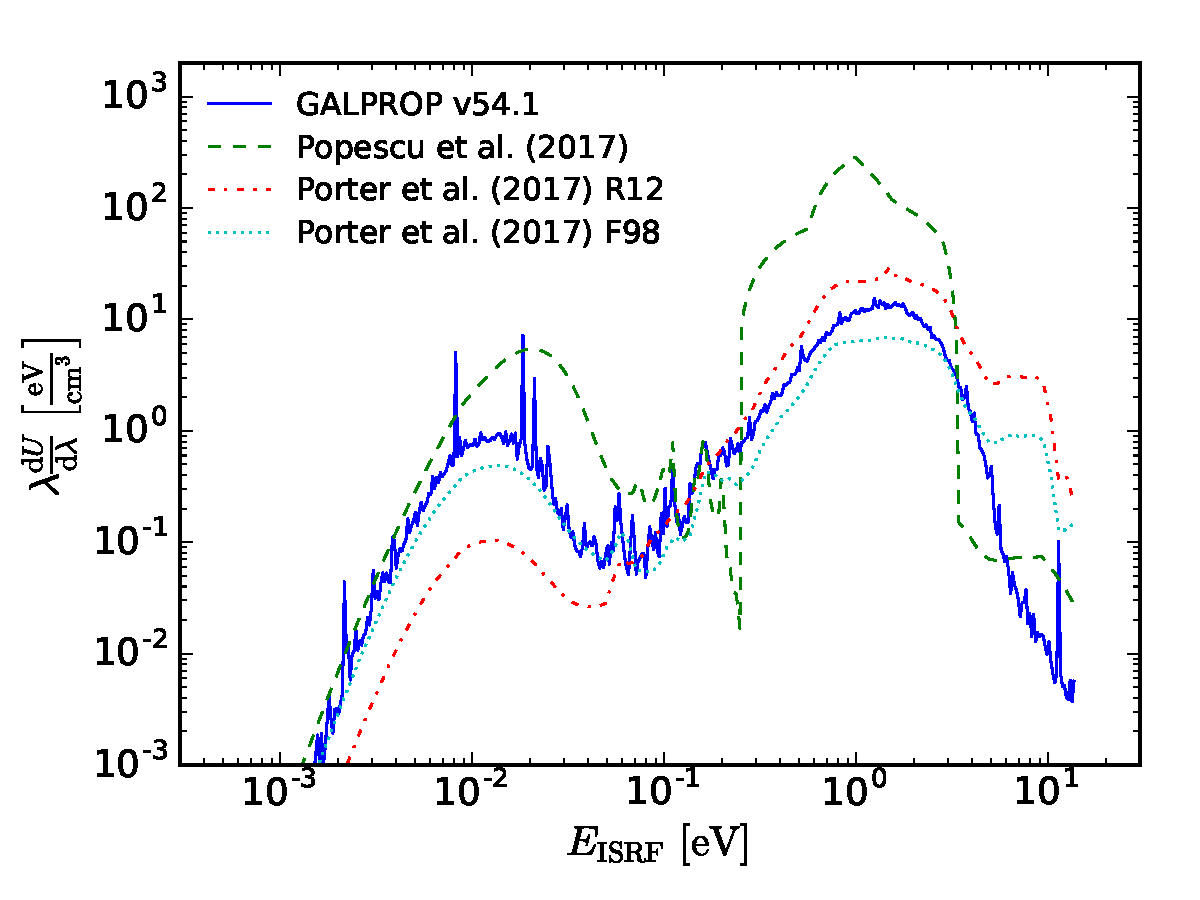
\includegraphics[width=\twopic\textwidth]{plots/ISRF_comparison}
\caption{Comparison of ISRF SEDs at the GC (see text for more details).}
\label{fig:isrfs}
\end{figure*}

In Figure \ref{fig:GC_CR} we show the IC models of the gamma-ray emission 
at the base of the FBs in the rectangle $b \in (-2\degr, 2\degr)$, $\ell \in (-10\degr, 0\degr)$
for the different ISRF models near the GC.
We separate the starlight (SL), infrared (IR) and cosmic microwave background (CMB) contributions.
The SL and IR ISRFs are separated by splitting the radiation field energy densities at 0.1 eV.
We model the CR electrons spectra by power-law function with an exponential cutoff.
We fix the cutoff at 1 PeV and fit the normalization and the spectral index by fitting 
the IC model to the \Fermi-LAT spectral points.
The corresponding parameters are presented in Table \ref{tab:CRe_syst}.
We use the GALPROP v54.1 ISRF as the reference model and show the normalizations of the CRe spectra
relative to the reference model (the normalizations are determined at 1 GeV).
The overall spread in the normalizations is about factor of 30,
while the variation of the index of the CRe spectra is less than 0.15.

\begin{figure*}[h]
\centering
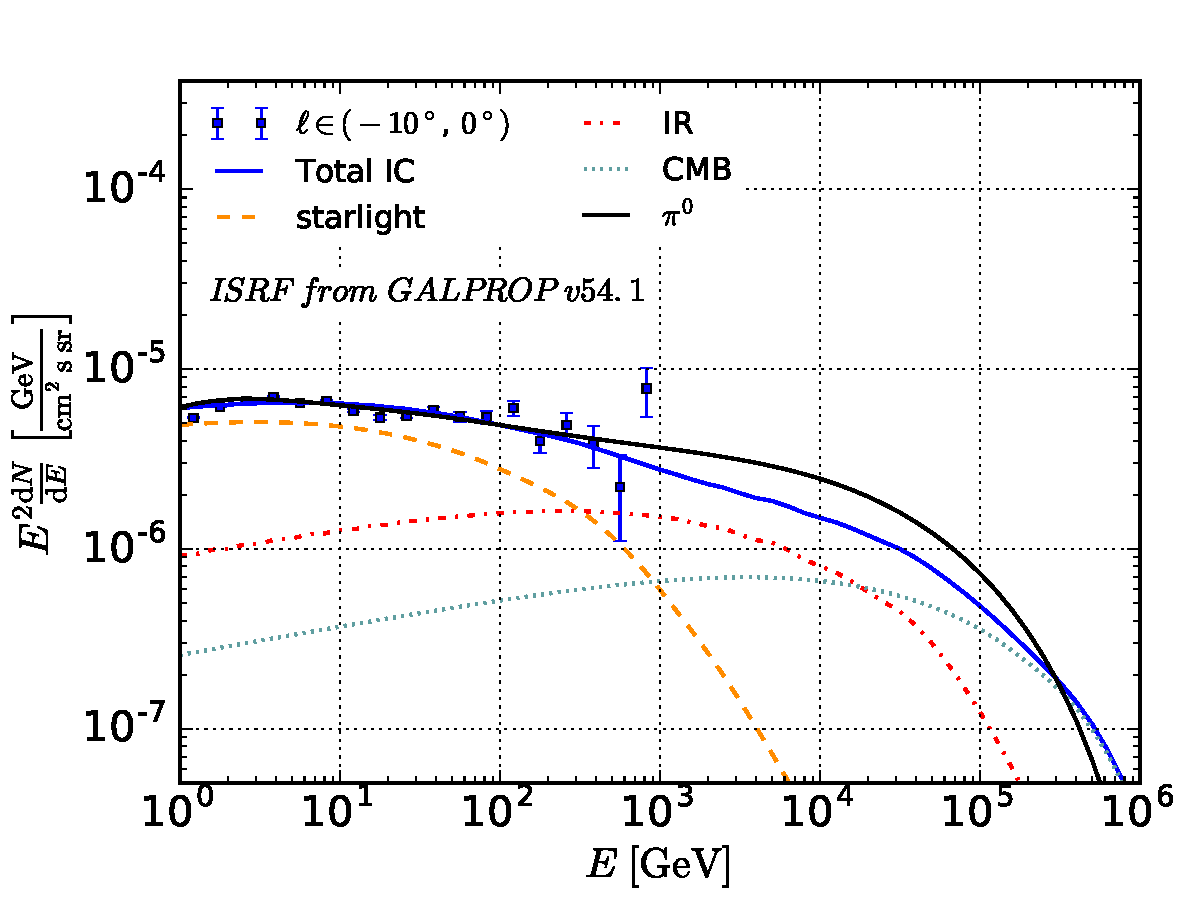
\includegraphics[width=\twopic\textwidth]{plots/SED_ISRF_componentsboxes_source_0_v54}
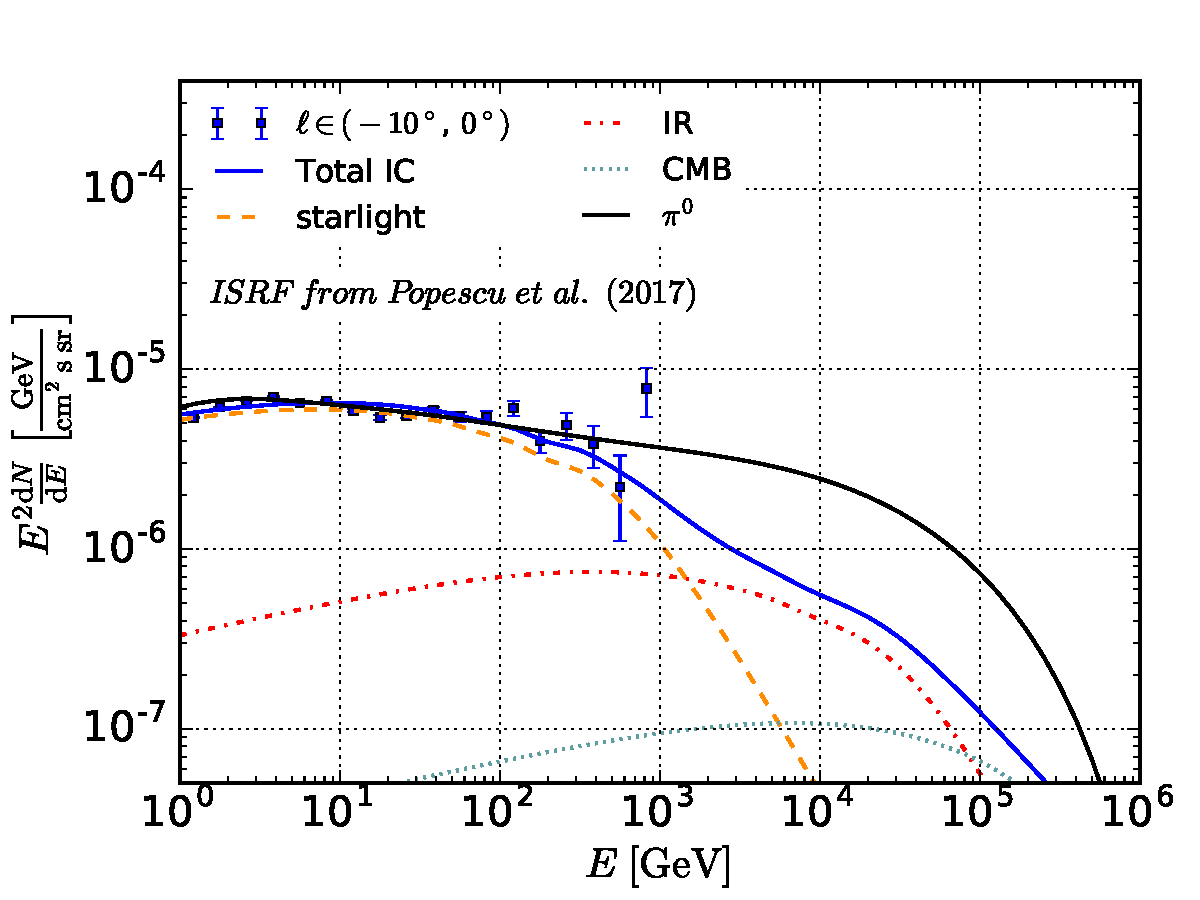
\includegraphics[width=\twopic\textwidth]{plots/SED_ISRF_componentsboxes_source_0_Popescu}
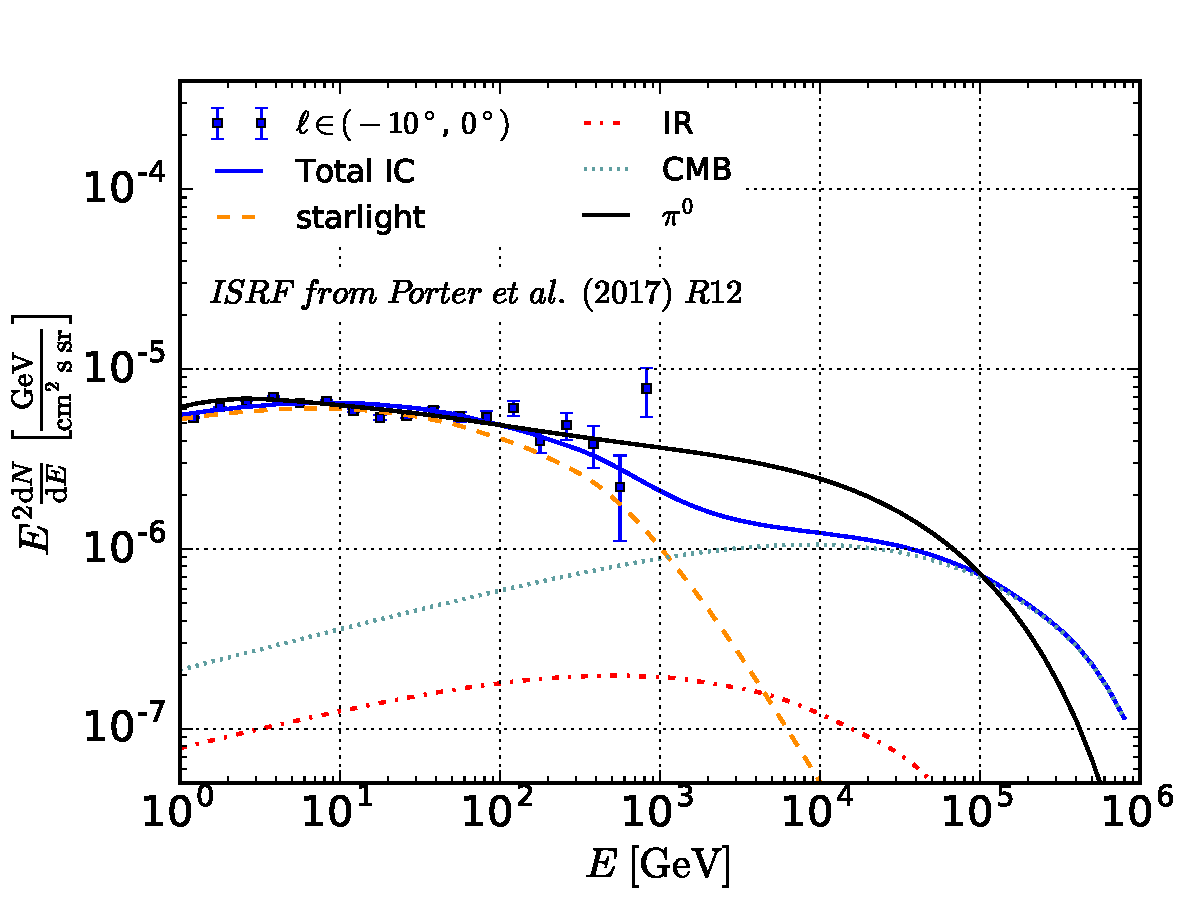
\includegraphics[width=\twopic\textwidth]{plots/SED_ISRF_componentsboxes_source_0_R12}
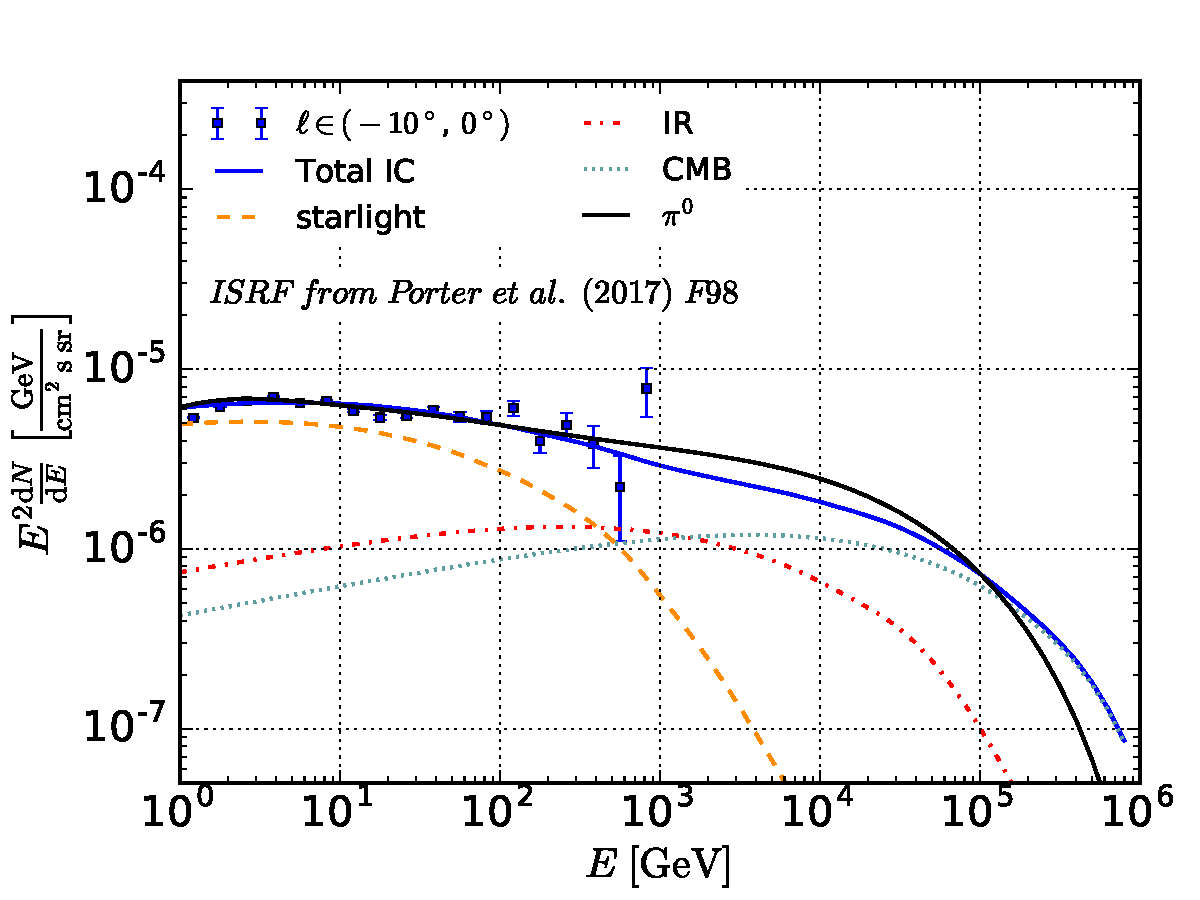
\includegraphics[width=\twopic\textwidth]{plots/SED_ISRF_componentsboxes_source_0_F98}
\caption{Contribution of different components of ISRFs to the IC model of the gamma-ray emission.
The data points correspond to the emission at the base of the FBs in the rectangle $b \in (-2\degr, 2\degr)$, $\ell \in (-10\degr, 0\degr)$
(middle panel in Figure \ref{fig:SED_with_fits}).
The spectrum of CR electrons is modeled by a power-law function with an exponential  cutoff at 1 PeV.
We separate the starlight and the IR contributions to the ISRF by formally splitting the ISRF at 0.1 eV.
The CR proton spectrum in the $\pi^0$ model of the gamma-ray emission
is modeled a power-law function with an exponential cutoff at 1 PeV.}
\label{fig:GC_CR}
\end{figure*}

\begin{table*}
  \begin{center}
    \caption{\label{tab:CRe_syst} 
Spectra of CR electrons near the GC relative to the reference model based on GALPROP v54.1 ISRF.
}
    \begin{tabular}{| l |c|c|} % <-- Alignments: 1st column left, 2nd middle and 3rd right, with vertical lines in between
     	\hline
		 ISRF model & Relative normalization at 1 GeV  & Index \\
		\hline
  		GALPROP v54.1 & 1 & 1.67 \\ 
  		\cite{2017ApJ...846...67P} R12 & 0.36 & 1.54 \\ 
  		\cite{2017ApJ...846...67P} F98 & 1.6 & 1.67 \\ 
  		\cite{2017MNRAS.470.2539P} & 0.057 & 1.58 \\ 
 \hline
    \end{tabular}
  \end{center}
\end{table*}




%\section{Details of the leptonic and hadronic models}
\lb{app:models}

The source function for the IC gamma rays is

\be
\label{eq:IC_spectrum}
E_\g\frac{\de Q_{\rm IC}}{\de E_\g} = c\int\!\! \int \left(\frac{\de n}{\de E}\right)_{\!\!\ISRF} \sigma_\IC\ \left(\frac{\de n}{\de E}\right)_{\!\!\el} \de E_\ISRF\, \de E_\el,
\ee
where $(\de n/ \de E)_\ISRF\ [\SI{}{GeV^{-1} cm^{-3}}]$ is the number density of ISRF photons,
$(\de n / \de E)_\el\ [\SI{}{GeV^{-1} cm^{-3}}]$ is the number density of electrons, and $\sigma_\IC(E_\gamma, E_\ISRF, E_\el)$
is the differential IC scattering cross section in units of $E_\g\frac{d\sigma}{d E_\g}$ \citep{1970RvMP...42..237B}.
\be
E^2 \frac{dF}{dE} = \frac{1}{4 \pi} \int E^2\frac{\de Q}{\de E} dR = 
\frac{Ec}{4\pi}\int \int \left(\frac{\de n}{\de E}\right)_{\!\!\ISRF} \sigma_\IC\ \left(\frac{\de \Sigma}{\de E}\right)_{\!\!\el} \de E_\ISRF\, \de E_\el,
\ee


The source function for the gamma rays is 
\be
\left(E\frac{\de Q}{\de E}\right)_{\!\!\gamma, \pi^0}\! = \int n_\Hy\ \sigma_\pr v_\pr \left(\frac{\de n}{\de T}\right)_{\!\!\pr} \de T_\pr,
\label{eq:had_spectrum}
\ee
where the integral goes over the kinetic energies of the protons $T_\pr = \sqrt{(qc)^2 + (mc^2)^2} - mc^2$,
$n_\Hy$ is the density of gas, and $\sigma_\pr (E_\gamma, T_\pr)$ is 
the differential cross section in units of $E_\g\frac{d\sigma}{d E_\g}$
for gamma rays in proton-proton collisions \citep{2006ApJ...647..692K, 2008ApJ...674..278K}.
We will use $n_\Hy = \SI{1}{cm^{-3}}$ as a characteristic density,
which is consistent with the gas surface density of $\sim 10 M_\odot {\rm pc}^{-2}$ \citep{2017ApJ...834...57M}
averaged over $\approx 200$ pc above and below the GC.

\end{appendix}

\end{document}

